\section{Queueing theoretic model}\label{sec:queueing-section}

One of the main outcomes of this research is the creation of a queueing network
model that consists of two queueing nodes and accepts two types of individuals.

\begin{figure}[h]
    \centering
    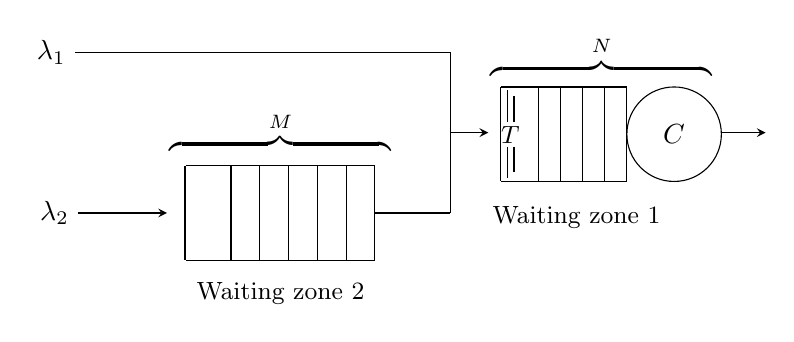
\begin{tikzpicture}[>=stealth, scale=0.8],
    % the rectangle of Queue 1
    \draw (0,0) -- ++(3cm,0) -- ++(0,-1.5cm) -- ++(-3cm,0);
    % The label above Queue 1 -> M
    \node[anchor=north] at (1.5cm, 1cm) {\(
        \overbrace{\qquad \qquad \qquad \qquad}^{M}
    \)};
    % The label below Queue 1 -> Waiting zone 2
    \node[anchor=north] at (1.5cm, -1.7cm) {\small{Waiting zone 2}};

    % the vertical lines in Queue 1
    \foreach \i in {1,...,5, 6.6}
    \draw (3cm-\i*13pt,0) -- +(0,-1.5cm);

    % % the circle in Queue 1
    % \draw (2.75,-0.75cm) circle [radius=0.75cm] node {\(0\)};

    % the rectangle in Queue 2
    \draw (5,1.25) -- ++(2cm,0) -- ++(0,-1.5cm) -- ++(-2cm,0);
    % the vertical lines in Queue 2
    \foreach \i in {1,...,4, 5.7}
    \draw (7cm-\i*10pt,1.25) -- +(0,-1.5cm);
    % The two vertical lines at the start of Queue 2
    \draw (7cm-54pt,1.2) -- +(0,-0.5cm);
    \draw (7cm-54pt,0.3) -- +(0,-0.5cm);
    \draw (7cm-51pt,1.1) -- +(0,-0.4cm);
    \draw (7cm-51pt,0.3) -- +(0,-0.4cm);

    % The label between the lines for T
    \node[anchor=north] at (5.15, 0.77 cm) {\small{\( T \)}};

    % The label above Queue 2 -> N
    \node[anchor=north] at (6.6cm, 2.2cm) {\(
        \overbrace{\qquad \qquad \qquad \qquad}^{N}
    \)};
    % The label below Queue 2 -> Waiting zone 1
    \node[anchor=north] at (6.2cm, -0.5cm) {\small{Waiting zone 1}};

    % the circle in Queue 2
    \draw (7.75,0.5) circle [radius=0.75cm] node {\(C\)};

    % Arrow line from Queue 2 outside
    \draw[->] (8.5,0.525) -- +(20pt,0);

    % Line from lambda_2 to Queue 1
    \draw[<-] (-0.3,-0.75) -- +(-40pt,0) node[left] {\( \lambda_2 \)};
    % First line (horizontal) after Queue 1
    \draw[-] (3,-0.75) -- +(34pt,0);
    % Second line (vertical) after Queue 1
    \draw (4.2, 0.525) -- (4.2, -0.75);

    % First line (horizontal) from lambda_1
    \draw (4.2, 1.8) -- +(-169.5pt,0) node[left] {\( \lambda_1 \)};
    % Second line (vertical) from lambda_1
    \draw (4.2, 1.8) -- (4.2, 0.525);
    % Arrow line to Queue 2
    \draw[->] (4.2, 0.525) -- (4.8, 0.525);
\end{tikzpicture}

    \caption{A diagrammatic representation of the queueing network.
    The threshold \(T\) only applies to type 2 individuals.
    If the number of individuals in node 1 is greater than or equal to
    \(T\), only individuals of type 1 are accepted (at a rate \(\lambda_1\))
    and individuals of type 2 (arriving at a rate \(\lambda_2\)) are blocked in
    node 2.}
    \label{fig:diagram_of_queueing_system}
\end{figure}

The model consists of two types of individuals; type 1 and type 2.
Type 1 individuals arrive instantly at node 1 and wait to receive their
service.
Type 2 individuals arrive at node 2 and wait there until they are
allowed to move to node 1.
They are allowed to proceed only when the number of
individuals in node 1 \textbf{and} in service is less than a
pre-determined threshold \(T\).
When the number of individuals is equal to or exceeds this threshold, all
type 2 individuals that arrive will stay \textit{blocked} in node 2
until the number of people in node 1 falls below \(T\).
This is shown diagrammatically in Figure~\ref{fig:diagram_of_queueing_system}.
The parameters of the described queueing model are:

\begin{itemize}
    \item \(\lambda_i\): The arrival rate of type \(i\) individuals where
    \(i\in\{1, 2\}\)
    \item \(\mu\): The service rate for individuals receiving service at
    node 1
    \item \(C\): The number of servers
    \item \(T\): The threshold at which individuals of the second type are
    blocked
    \item \(N\): The capacity of node 1 (i.e \(N=C + 
    \text{(Queue capacity)}\))
    \item \(M\): The capacity of node 2
\end{itemize}

In chapter ?
% TODO: reference chapter \ref{ch:ed-ems-application}
this queueing network will be used to model the emergent behaviour between
Emergency Departments (EDs) and the Emergency Medical Systems (EMS).


\subsection{Discrete Event Simulation}\label{sec:discrete_event_simulation}

Discrete Event Simulation (DES) is a method for modelling the behaviour of
real-world systems in which the system is made up of discrete events, each of
which has a certain duration~\cite{DESstewart}.
It can be used to understand complex situations in order to make predictions
and thus provide improvements~\cite{VinceGeraintBook}.
The three main approaches to building DES models are the activity scanning
approach, the event scheduling approach and the process interaction
approach~\cite{DESapproaches}.
Under the scope of this study only the event scheduling approach is considered.
This section describes the discrete event simulation (DES) model used to
represent the queueing network of Section~\ref{sec:queueing-section}.

In order to use DES on the queueing network described in
Figure~\ref{fig:diagram_of_queueing_system} an equivalent queueing network must
be constructed.
The current queueing network is a two-node queueing system that accepts two
types of individuals, where type 1 individuals arrive at node 1 and
type 2 individuals arrive at node 2.
The modification that is required revolves around the mechanisms of node 2.
Node 2 is defined as a non-service node where there is only a queueing
space for individuals to wait there until they are allowed to node 1.
From an implementation perspective there is an equivalent system that can be
used where instead of a node with no service and queueing capacity \(M\), there
are \(M\) servers each serving with a service rate of \(0\) and no queueing
capacity, as shown in Figure~\ref{fig:equivalent_diagram_of_queueing_system}.

\begin{figure}[H]
    \centering
    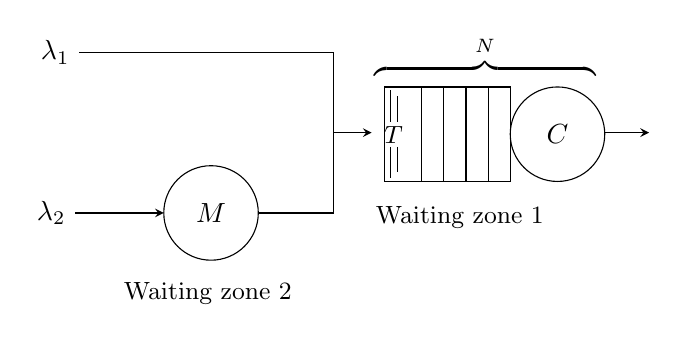
\begin{tikzpicture}[>=stealth, scale=0.8],

    % the circle in Queue 1
    \draw (2.25cm, -0.75cm) circle [radius=0.75cm] node {\(M\)};

    % The label below Queue 1 -> Waiting zone 2
    \node[anchor=north] at (2.2cm, -1.7cm) {\small{Waiting zone 2}};

    % the rectangle in Queue 2
    \draw (5, 1.25) -- ++(2cm, 0) -- ++(0, -1.5cm) -- ++(-2cm, 0);
    % the vertical lines in Queue 2
    \foreach \i in {1,...,4, 5.7}
    \draw (7cm-\i*10pt,1.25) -- +(0,-1.5cm);
    % The two vertical lines at the start of Queue 2
    \draw (7cm-54pt,1.2) -- +(0,-0.5cm);
    \draw (7cm-54pt,0.3) -- +(0,-0.5cm);
    \draw (7cm-51pt,1.1) -- +(0,-0.4cm);
    \draw (7cm-51pt,0.3) -- +(0,-0.4cm);

    % The label between the lines for T
    \node[anchor=north] at (5.15, 0.77 cm) {\small{\( T \)}};

    % The label above Queue 2 -> N
    \node[anchor=north] at (6.6cm, 2.2cm) {\(
        \overbrace{\qquad \qquad \qquad \qquad}^{N}
    \)};
    % The label below Queue 2 -> Waiting zone 1
    \node[anchor=north] at (6.2cm, -0.5cm) {\small{Waiting zone 1}};

    % the circle in Queue 2
    \draw (7.75,0.5) circle [radius=0.75cm] node {\(C\)};

    % Arrow line from Queue 2 outside
    \draw[->] (8.5,0.525) -- +(20pt,0);

    % Line from lambda_2 to Queue 1
    \draw[<-] (1.5,-0.75) -- +(-40pt,0) node[left] {\( \lambda_2 \)};
    % First line (horizontal) after Queue 1
    \draw[-] (3,-0.75) -- +(34pt,0);
    % Second line (vertical) after Queue 1
    \draw (4.2, 0.525) -- (4.2, -0.75);

    % First line (horizontal) from lambda_1
    \draw (4.2, 1.8) -- +(-115pt,0) node[left] {\( \lambda_1 \)};
    % Second line (vertical) from lambda_1
    \draw (4.2, 1.8) -- (4.2, 0.525);
    % Arrow line to Queue 2
    \draw[->] (4.2, 0.525) -- (4.8, 0.525);
\end{tikzpicture}

    \caption{An equivalent model to the one described in
    Figure~\ref{fig:diagram_of_queueing_system}. The difference between the two
    diagrams is the formulation of node 2. The original diagram uses
    a node with no servers and a queueing capacity of \(M\) while this one uses
    \(M\) servers with no queueing capacity.}
    \label{fig:equivalent_diagram_of_queueing_system}
\end{figure}
    

The arrival times for both nodes are exponentially distributed with
mean \(\lambda_1\) and \(\lambda_2\) corresponding to type 1 and type 2
individuals respectively.
Node 1 has an exponentially distributed service time with rate \(\mu\),
a total of \(C\) servers and a queueing capacity of \(N - C\) (making the
overall capacity \(N\)). 
Node 2 has a deterministic service time of \(0\), a total of \(M\)
servers and a queueing capacity of \(M\).
Note here that, similar to Figure \ref{fig:diagram_of_queueing_system},
parameters \(N\) and \(M\) are used to approximate the real world system 
and in fact can be taken to be infinite in the DES.
Finally the routing parameter is defined as an array that probabilistically
routes individuals from all nodes to all other nodes.
For this particular system the routing parameter needs only to route individuals
from node 2 to node 1.

\begin{equation}
    \text{routing parameter} = \left[
    \begin{array}{cc}
        0 & 1 \\
        0 & 0
    \end{array}
    \right]
\end{equation}


\subsubsection{Implementation}
The python library \lstinline[style=pystyle]{ciw}~\cite{ciwpython, ciwarticle}
was used to implement the DES model.
The library treats queues as distinct nodes in the network where each node has
an arrival distribution, a service distribution, a number of available servers
and a queue capacity.

The following code can be used to generate a queueing network with two
queues and two types of individuals, where type 1 individuals arrive at node
1 with an arrival rate of \lstinline[style=pystyle]{lambda_1} and type 2
individuals arrive at node 2 with an arrival rate of
\lstinline[style=pystyle]{lambda_2}.
Node 2 has a deterministic fixed service rate of
\lstinline[style=pystyle]{0} (since there is no service involved in the buffer
centre) and node 1 has an exponential service rate of
\lstinline[style=pystyle]{mu}.

\begin{lstlisting}[style=pystyle]
>>> import ciw
>>> lambda_1 = 1.0
>>> lambda_2 = 2.0
>>> mu = 0.5
>>> num_of_servers = 3
>>> system_capacity = 10
>>> buffer_capacity = 5
>>> model = ciw.create_network(
...     arrival_distributions=[
...         ciw.dists.Exponential(lambda_2),
...         ciw.dists.Exponential(lambda_1)
...     ],
...     service_distributions=[
...         ciw.dists.Deterministic(0), ciw.dists.Exponential(mu)
...     ],
...     routing=[
...         [0.0, 1.0],
...         [0.0, 0.0]
...     ],
...     number_of_servers=[buffer_capacity, num_of_servers],
...     queue_capacities=[0, system_capacity - num_of_servers],
... )

\end{lstlisting}

As described earlier in Section~\ref{sec:queueing-section} and as shown in
Figure~\ref{fig:diagram_of_queueing_system}, type 1 individuals arrive at
node 1 and exit the system after their service finishes, but type 2 individuals
arrive at node 2 and then proceed to node 1 after leaving node 2.
This logic is implemented in the queueing network using the
\lstinline[style=pystyle]{routing} parameter that consists of the routing
probabilities between different nodes.
For the current implementation the routing matrix is a \(2 \times 2\) array
that routes individuals from node 2 to node 1 with a probability of
\(1.0\).
Furthermore, the server availability for nodes 1 and 2 are set to
the \lstinline[style=pystyle]{buffer_capacity} and
\lstinline[style=pystyle]{num_of_servers} respectively and the queue capacities
are set to \lstinline[style=pystyle]{0} and
\lstinline[style=pystyle]{system_capacity - num_of_servers}.
Note that for node 2 queue capacity is set to 0 and its
number of servers is set to the buffer capacity.
From \lstinline[style=pystyle]{ciw}'s data records perspective this made more
sense since individuals are recorded as blocked this way.
If the queue capacity was non-zero, individuals could also have a waiting time
but no waiting should take place in node 2, only blockage.


\subsubsection{Custom node class}
Another specific feature of the particular model is that type 2 individuals
need to stay blocked in node 2 whenever the number of individuals in node 1
reaches a certain threshold \(T\).
This part of the queueing network is not as straightforward to implement as the
rest of the model.
\lstinline[style=pystyle]{Ciw} allows users to get more custom behaviour by
creating their own node class that inherits from the original one.
By inheriting the original \lstinline[style=pystyle]{ciw.Node} the general
behaviour of all nodes can be altered.
Note that node ids are assigned in the order they are created so in the
\lstinline[style=pystyle]{ciw} implementation node 2 is assigned id 1 and node 1
is assigned id 2.


\begin{lstlisting}[style=pystyle]
>>> import numpy as np
>>> def build_custom_node(threshold=float("inf")):
...     """
...     Build a custom node to replace the default ciw.Node. Inherits from
...     the original ciw.Node class and replaces methods
...     release_blocked_individual and finish_service.
...     The methods are modified in such a way that all individuals that
...     are in the buffer space (node 1) stay blocked as long as the
...     number of individuals in the service area node (node 2) exceeds the
...     threshold.
...
...     Parameters
...     ----------
...     threshold : int, optional
...         The capacity threshold to be used by the method
...     Returns
...     -------
...     class
...         A custom node class that inherits from ciw.Node
...     """
...
...     class CustomNode(ciw.Node):
...         """
...         Overrides the default release_blocked_individual and
...         finish_service methods of the ciw.Node class
...         """
...
...         def __init__(self, id_, simulation):
...             """
...             Initializes the node with the given id and simulation using
...             the initialisation of ciw's Node object with the addition of
...             the threshold parameter.
...             """
...             super().__init__(id_, simulation)
...             self.simulation.threshold = threshold
...
...         def release_blocked_individual(self):
...             """
...             Releases an individual who becomes unblocked when
...             another individual is released:
...             - check if individual in node 2 and should stay blocked
...                 i.e. if the number of individuals in that
...                      node > threshold
...             - check if anyone is blocked by this node
...             - find the individual who has been blocked the longest
...             - remove that individual from blocked queue
...             - check if that individual had their service interrupted
...             - release that individual from their node
...             """
...             continue_blockage = (
...                 self.number_of_individuals >= threshold
...                 and self.id_number == 2
...             )
...             if (
...                 self.len_blocked_queue > 0
...                 and self.number_of_individuals < self.node_capacity
...                 and not continue_blockage
...             ):
...                 receiving_node = (
...                     self.simulation.nodes[self.blocked_queue[0][0]]
...                 )
...                 individual_to_receive_index = [
...                     ind.id_number
...                     for ind in receiving_node.all_individuals
...                 ].index(self.blocked_queue[0][1])
...                 individual_to_receive = (
...                     receiving_node.all_individuals[
...                         individual_to_receive_index
...                     ]
...                 )
...                 self.blocked_queue.pop(0)
...                 self.len_blocked_queue -= 1
...                 if individual_to_receive.interrupted:
...                     individual_to_receive.interrupted = False
...                     receiving_node.interrupted_individuals.remove(
...                         individual_to_receive
...                     )
...                     receiving_node.number_interrupted_individuals -= 1
...                 receiving_node.release(individual_to_receive_index, self)
...
...         def finish_service(self):
...             """
...             The next individual finishes service:
...             - finds the individual to finish service
...             - check if they need to change class
...             - find their next node
...             - release the individual if there is capacity at destination,
...                 otherwise cause blockage
...             - Note that blockage also occurs when we are at node 1 and
...                 the number of individuals on node 2 are more than the
...                 'threshold'
...             """
...             (
...                 next_individual,
...                 next_individual_index
...             ) = self.find_next_individual()
...             self.change_customer_class(next_individual)
...             next_node = self.next_node(next_individual)
...             next_individual.destination = next_node.id_number
...             if not np.isinf(self.c):
...                 next_individual.server.next_end_service_date=float("Inf")
...             blockage = (
...                 next_node.number_of_individuals >= threshold
...                 and self.id_number == 1
...             )
...             if (
...                 next_node.number_of_individuals < next_node.node_capacity
...             ) and not blockage:
...                 self.release(next_individual_index, next_node)
...             else:
...                 self.block_individual(next_individual, next_node)
...
...     return CustomNode

\end{lstlisting}

The class \lstinline[style=pystyle]{CustomNode} inherits from
\lstinline[style=pystyle]{ciw.Node} and changes two of the methods
(\lstinline[style=pystyle]{release_blocked_individual} and
\lstinline[style=pystyle]{finish_service}) so that the additional logic of the
threshold is incorporated.
In the \lstinline[style=pystyle]{release_blocked_individual} method an
additional check is added before releasing a potentially blocked individual from
node 2 to node 1.
This essentially checks whether the id number of the node is 2 and
the number of individuals in it are more than or equal to the
\lstinline[style=pystyle]{threshold} so that it can accept a blocked individual.
Similarly \lstinline[style=pystyle]{finish_service} is called once an individual
finishes their service.
The additional check that was added checks whether the id of the node is 1 and
the number of individuals in the next node (i.e. node 1) is more than the
threshold, which would result in blockage.
Finally, the simulation object can be created and simulated for a specific
\lstinline[style=pystyle]{threshold} and \lstinline[style=pystyle]{runtime} by
running:

\begin{lstlisting}[style=pystyle]
>>> threshold = 4
>>> runtime = 1000
>>> custom_node = build_custom_node(threshold)
>>> ciw.seed(0)
>>> simulation = ciw.Simulation(model, node_class=custom_node)
>>> simulation.simulate_until_max_time(runtime)

\end{lstlisting}


\subsubsection{Performance Measures}

Having run the simulation using \lstinline[style=pystyle]{ciw} all necessary
performance measures can be calculated.
All performance measure that are related to the duration of time are relatively
straightforward to calculate.
The following code gets all waiting times, service times and blocking times for
all individuals that have passed through the model.

\begin{lstlisting}[style=pystyle]
>>> def extract_times_from_records(simulation_records, warm_up_time):
...     """Get the required times (waiting, service, blocking) out of ciw's
...     records where all individuals are treated the same way. This function
...     can't distinguish between class 1 and class 2 individuals. It returns
...     the aggregated waiting time, service times BUT only blocking times of
...     class 2 individuals.
...     """
...     waiting_times = [
...         r.waiting_time
...         for r in simulation_records
...         if r.arrival_date > warm_up_time and r.node == 2
...     ]
...     serving_times = [
...         r.service_time
...         for r in simulation_records
...         if r.arrival_date > warm_up_time and r.node == 2
...     ]
...     blocking_times = [
...         r.time_blocked
...         for r in simulation_records
...         if r.arrival_date > warm_up_time and r.node == 1
...     ]
...     return waiting_times, serving_times, blocking_times

\end{lstlisting}

Using the earlier variable \lstinline[style=pystyle]{simulation}, the waiting
times, service times and blocking times can be extracted from the simulation
records.

\begin{lstlisting}[style=pystyle]
>>> warm_up_time = 100
>>> all_records = simulation.get_all_records()
>>> waiting_times, serving_times, blocking_times = extract_times_from_records(
...     all_records, warm_up_time
... )
>>> np.mean(waiting_times), np.mean(serving_times), np.mean(blocking_times)
(1.7038750111337655, 2.041619227158985, 8.227702587974997)

\end{lstlisting}


\subsection{Markov chain model}

A Markov chain is a stochastic model that is the primary analytical tool to
study queues.
Under the assumption that all rates (arrival and service) are Markovian the
queueing system can be represented by a Markov chain
model~\cite{kemeny1976markov}.
The states of the Markov chain are denoted by \((u,v)\) where:

\begin{itemize}
    \item \(u\) is the number of individuals blocked in node 2
    \item \(v\) is the number of individuals either in node 1 or in the
    service centre
\end{itemize}

The set of all possible combination of pairs \((u, v)\) form all the possible
states that the system can visit.
The state space of the Markov chain is denoted as the set \(S=S(T)\) which can
be written as the disjoint union:

\begin{align}
    S(T) =& S_1(T) \cup S_2(T) \text{ where:} \nonumber \\
    S_1(T) =& \left\{(0, v)\in\mathbb{N}_0^2 \; | \; v < T \right\}
    \label{eq:definition_of_S_as_disjoint_union} \\
    S_2(T) =& \{(u, v)\in\mathbb{N}_0^2 \; | \; v \geq T \} \nonumber
\end{align}

\(S_1\) consists of the set of states where the number of individuals in node
is less than \(T\) (i.e. \(v < 0\)) and subsequently the number of
individuals in node 2 is zero (i.e. \(u = 0\)).
Similarly, \(S_2\) consists of the set of states where the number of individuals
in node 1 is greater than or equal to \(T\) (i.e. \(v \geq T\)) and
hence it is possible for individuals to be at node 2 (i.e.
\(u \geq 0\)).
This is illustrated diagrammatically in Figure~\ref{fig:general_markov_model}.

Having defined the set of states of the Markov chain model, the generator
matrix can also be obtained.
The generator matrix \(Q\) of the Markov chain consists of the
rates between the numerous states of the model.
Every entry \( Q_{ij} = Q_{(u_i, v_i),(u_j, v_j)} \) represents the rate from
state \( i = (u_i, v_i) \) to state \( j = (u_j , v_j) \) for all
\( (u_i, v_i), (u_j, v_j) \in S \).
The entries of \(Q\) can be calculated using the state-mapping function
described in equation (\ref{eq:markov_transition_rate}).
Here \(\Lambda\) denotes the overall arrival rate in the model for
both types of individuals (i.e. \(\Lambda = \lambda_1 + \lambda_2\)).

\begin{equation} \label{eq:markov_transition_rate}
    Q_{ij} =
    \begin{cases}
        \Lambda, & \textbf{if } (u_i, v_i) - (u_j, v_j) = (0,-1) \textbf{ and }
        v_i < \text{t} \\
        \lambda_1, & \textbf{if } (u_i, v_i) - (u_j, v_j) = (0,-1)
        \textbf{ and } v_i \geq \text{t} \\
        \lambda_2, & \textbf{if } (u_i, v_i) - (u_j, v_j) = (-1,0) \\
        v_i \mu, & \textbf{if } (u_i, v_i) - (u_j, v_j) = (0,1) \textbf{ and }
        v_i \leq C \textbf{ or} \\ & \hspace{0.37cm}(u_i, v_i) - (u_j, v_j) =
        (1,0) \textbf{ and } v_i = T \leq C \\
        C \mu, & \textbf{if } (u_i, v_i) - (u_j, v_j) = (0,1) \textbf{ and }
        v_i > C
        \textbf{ or} \\ & \hspace{0.37cm}(u_i, v_i) - (u_j, v_j) = (1,0)
        \textbf{ and } v_i = T > C\\
        -\sum_{j=1}^{|Q|}{Q_{ij}} & \textbf{if } i = j \\
        0, & \textbf{otherwise}
    \end{cases}
\end{equation}

Note that for large values of \(N\) and \(M\) most of the entries of the
transition matrix will be zero.
In order to speed up the computation of the transition matrix, instead of
considering every possible pair of states in the state space a new function
that maps a state to every possible destination state can be used.
Function \(\mathcal{M}\) from equation (\ref{eq:state_map_to_destination_states})
takes a state \((u, v)\) and maps it to the set of
all possible destination states that the system can go to when on that state.

\begin{equation}\label{eq:state_map_to_destination_states}
    \mathcal{M}(u, v) =
    \begin{cases}
        \{(u, v + 1), (u, v - 1)\} & \textbf{if } v < T \\
        \{(u + 1, v), (u, v + 1), (u, v - 1)\} & \textbf{if } v = T
        \textbf{ and } u = 0 \\
        \{(u + 1, v), (u, v + 1), (u - 1, v)\} & \textbf{if } v = T
        \textbf{ and } u > 0 \\
        \{(u, v + 1), (u + 1, v), (u, v - 1)\} & \textbf{if } v > T \\
    \end{cases}
\end{equation}


A visualisation of how the transition rates relate to the states of the model
can be seen in the general Markov chain model shown in
Figure~\ref{fig:general_markov_model}.

\begin{figure}[H]
    \centering
    \scalebox{.8}
    {\begin{tikzpicture}[-, node distance = 0.9cm, auto, every node/.style={scale=0.7}]

    % Markov chain variables
    \tikzmath{
        let \initdist = 0.5cm;
        let \altdist = 1.2cm;
        let \minsz = 1.6cm;
    }

    % S_1 and S_2 rectangles
    \tikzmath{
        let \leftOne = -0.8;
        let \rightOne = 2.7;
        let \upOne = 0.8;
        let \downOne = -2.7;
        let \leftTwo = 2.8;
        let \rightTwo = 13;
        let \upTwo = -2.90;
        let \downTwo = -16.8;
    }

    % General case variables
    \tikzmath{
        let \GCsmallx = 8.3;
        let \GCsmally = -9.5;
        let \GCbigx = 4.2;
        let \GCbigy = -12;
    }

    % Rectangle for S1
    \draw[ultra thin, dashed] (\leftOne, \downOne) -- (\leftOne, \upOne);
    \draw[ultra thin, dashed] (\leftOne, \upOne) -- (\rightOne, \upOne);
    \draw[ultra thin, dashed] (\rightOne, \upOne) -- node 
    {\Huge{\( \quad S_1 \)}}(\rightOne, \downOne);
    \draw[ultra thin, dashed] (\rightOne, \downOne) -- (\leftOne, \downOne);

    % Rectangle for S2
    \draw[ultra thin, dashed] (\leftTwo, \downTwo) -- node 
    {\Huge{\( S_2 \quad \)}}(\leftTwo, \upTwo);
    \draw[ultra thin, dashed] (\leftTwo, \upTwo) -- (\rightTwo, \upTwo);
    \draw[ultra thin, dashed] (\rightTwo, \upTwo) -- (\rightTwo, \downTwo);
    \draw[ultra thin, dashed] (\rightTwo, \downTwo) -- (\leftTwo, \downTwo);

    % Small square of general case
    \draw [thick] (\GCsmallx, \GCsmally) -- node {} 
    (\GCsmallx + 0.4, \GCsmally);
    \draw [thick] (\GCsmallx + 0.4, \GCsmally) -- node {} 
    (\GCsmallx + 0.4, \GCsmally - 0.4);
    \draw [thick] (\GCsmallx + 0.4, \GCsmally - 0.4) -- node {} 
    (\GCsmallx, \GCsmally - 0.4);
    \draw [thick] (\GCsmallx, \GCsmally - 0.4) -- node {} 
    (\GCsmallx, \GCsmally);


    % Dashed lines to from small square to big one 
    \draw [ultra thin] (\GCsmallx, \GCsmally) -- node {} 
    (\GCbigx, \GCbigy);
    \draw [ultra thin] (\GCsmallx + 0.4, \GCsmally) -- node {} 
    (\GCbigx + 4, \GCbigy);
    \draw [ultra thin] (\GCsmallx, \GCsmally - 0.4) -- node {} (7, \GCbigy);
    \draw [ultra thin] (\GCsmallx + 0.4, \GCsmally - 0.4) -- node {} 
    (\GCbigx + 4, \GCbigy - 4);
    
    % Big Square of general case
    \draw [ultra thick] (\GCbigx, \GCbigy) -- node {} (\GCbigx + 4, \GCbigy);
    \draw [ultra thick] (\GCbigx + 4, \GCbigy) -- node {} 
    (\GCbigx + 4, \GCbigy - 4);
    \draw [ultra thick] (\GCbigx + 4, \GCbigy - 4) -- node {General Case} 
    (\GCbigx, \GCbigy - 4);
    \draw [ultra thick] (\GCbigx, \GCbigy - 4) -- node {} (\GCbigx, \GCbigy);

    % First Line
    \node[state, minimum size=\minsz] (zero) {(0,0)};
    \node[state, node distance = \initdist, minimum size=\minsz, below right=of zero] 
    (one) {(0,1)};
    \node[draw=none, node distance = \initdist, minimum size=\minsz, below right=of one] 
    (two) {\textbf{\( \ddots \)}};
    \node[state, node distance = \initdist, minimum size=\minsz, below right=of two] 
    (three) {(0,T)};
    \node[state, node distance = \altdist, minimum size=\minsz, right=of three] 
    (four) {\footnotesize(0,T+1)};
    \node[draw=none, node distance = \altdist, minimum size=\minsz, right=of four] 
    (five) {\textbf{\dots}};
    \node[state, minimum size=\minsz, right=of five] (six) {(0,C)};
    \node[draw=none, minimum size=\minsz, right=of six] (seven) {\textbf{\dots}};

    % Second Line
    \node[state, minimum size=\minsz, below=of three] (three_one) {(1,T)};
    \node[state, minimum size=\minsz, below=of four] (four_one) {\footnotesize(1,T+1)};
    \node[draw=none, minimum size=\minsz, below=of five] (five_one) {\textbf{\dots}};
    \node[state, minimum size=\minsz, right=of five_one] (six_one) {(1,C)};
    \node[draw=none, minimum size=\minsz, right=of six_one] (seven_one) {\textbf{\dots}};
    
    % Third Line
    \node[state, minimum size=\minsz, below=of three_one] (three_two) {(2,T)};
    \node[state, minimum size=\minsz, below=of four_one] (four_two) {\footnotesize(2,T+1)};
    \node[draw=none, minimum size=\minsz, below=of five_one] (five_two) 
    {\textbf{\dots}};
    \node[state, minimum size=\minsz, right=of five_two] (six_two) {(2,C)};
    \node[draw=none, minimum size=\minsz, right=of six_two] (seven_two) 
    {\textbf{\dots}};

    % Fourth line
    \node[draw=none, node distance = \altdist, minimum size=\minsz, below=of three_two] 
    (three_three) {\textbf{\vdots}};
    \node[draw=none, node distance = \altdist, minimum size=\minsz, below=of four_two] 
    (four_three) {\textbf{\vdots}};
    \node[draw=none, node distance = 2cm, minimum size=\minsz, below=of five_two] 
    (five_three) {};
    \node[draw=none, node distance = \altdist, minimum size=\minsz, below=of six_two] 
    (six_three) {\textbf{\vdots}};

    % Fifth line
    \node[draw=none, node distance = 0.3cm, minimum size=\minsz, below=of four_three] 
    (general_case_up) {};
    \node[state, node distance = \altdist, minimum size=\minsz, below=of general_case_up] 
    (general_case_mid) {\( (u_i, v_i) \)};

    \node[draw=none, node distance = \altdist, minimum size=\minsz, below=of general_case_mid] 
    (general_case_down) {};
    \node[draw=none, node distance = \altdist, minimum size=\minsz, left=of general_case_mid] 
    (general_case_left) {};
    \node[draw=none, node distance = \altdist, minimum size=\minsz, right=of general_case_mid] 
    (general_case_right) {};

    \draw[every loop]
        % First Horizontal Edges
        (zero) edge[bend left] node {\( \Lambda \)} (one)
        (one) edge[bend left] node {\( \mu \)} (zero)
        (one) edge[bend left] node {\( \Lambda \)} (two)
        (two) edge[bend left] node {\( 2 \mu \)} (one)
        (two) edge[bend left] node {\( \Lambda \)} (three)
        (three) edge[bend left] node {\( T \mu \)} (two)
        (three) edge[bend left] node {\( \lambda_1 \)} (four)
        (four) edge[bend left] node {\( (T+1) \mu \)} (three)
        (four) edge[bend left] node {\( \lambda_1 \)} (five)
        (five) edge[bend left] node {\( (T+2) \mu \)} (four)
        (five) edge[bend left] node {\( \lambda_1 \)} (six)
        (six) edge[bend left] node {\( C\mu \)} (five)
        (six) edge[bend left] node {\( \lambda_1 \)} (seven)
        (seven) edge[bend left] node {\( C\mu \)} (six)

        % Second Horizontal Edges
        (three_one) edge[bend left] node {\( \lambda_1 \)} (four_one)
        (four_one) edge[bend left] node {\( (T+1) \mu \)} (three_one)
        (four_one) edge[bend left] node {\( \lambda_1 \)} (five_one)
        (five_one) edge[bend left] node {\( (T+2) \mu \)} (four_one)
        (five_one) edge[bend left] node {\( \lambda_1 \)} (six_one)
        (six_one) edge[bend left] node {\( C\mu \)} (five_one)
        (six_one) edge[bend left] node {\( \lambda_1 \)} (seven_one)
        (seven_one) edge[bend left] node {\( C\mu \)} (six_one)

        % Third Horizontal Edges
        (three_two) edge[bend left] node {\( \lambda_1 \)} (four_two)
        (four_two) edge[bend left] node [below] {\( (T+1) \mu \)} (three_two)
        (four_two) edge[bend left] node {\( \lambda_1 \)} (five_two)
        (five_two) edge[bend left] node {\( (T+2) \mu \)} (four_two)
        (five_two) edge[bend left] node {\( \lambda_1 \)} (six_two)
        (six_two) edge[bend left] node {\( C\mu \)} (five_two)
        (six_two) edge[bend left] node {\( \lambda_1 \)} (seven_two)
        (seven_two) edge[bend left] node {\( C\mu \)} (six_two)

        % First Vertical Edges
        (three) edge[bend left] node {\( \lambda_2 \)} (three_one)
        (three_one) edge[bend left] node {\( T \mu \)} (three)
        (three_one) edge[bend left] node {\( \lambda_2 \)} (three_two)
        (three_two) edge[bend left] node {\( T\mu \)} (three_one)
        (three_two) edge[bend left] node {\( \lambda_2 \)} (three_three)
        (three_three) edge[bend left] node {\( T\mu \)} (three_two)

        % Second Vertical Edges
        (four) edge node {\( \lambda_2 \)} (four_one)
        (four_one) edge node {\( \lambda_2 \)} (four_two)
        (four_two) edge node {\( \lambda_2 \)} (four_three)

        % Fourth Vertical Edges
        (six) edge node {\( \lambda_2 \)} (six_one)
        (six_one) edge node {\( \lambda_2 \)} (six_two)
        (six_two) edge node {\( \lambda_2 \)} (six_three)

        % General Case
        (general_case_left) edge[bend left] node {\( \lambda_1 \)} (general_case_mid)
        (general_case_mid) edge[bend left] node {\( v_i \mu \)} (general_case_left)
        (general_case_right) edge[bend left] node {\( (v_i +1) \mu \)} (general_case_mid)
        (general_case_mid) edge[bend left] node {\( \lambda_1 \)} (general_case_right)
        % (five_three) edge node {\( \lambda_2 \)} (general_case_mid)
        (general_case_up) edge node {\( \lambda_2 \)} (general_case_mid)
        (general_case_mid) edge node {\( \lambda_2 \)} (general_case_down)
        ;
\end{tikzpicture}
}
    \caption{General case of the Markov chain model} 
    \label{fig:general_markov_model}
\end{figure}


In order to consider this model numerically an adjustment needs to be made.
The problem defined above assumes no upper boundary to the number of individuals
that can wait for service or for the ones that are blocked in node 2.
Therefore, a different state space \( \tilde S \) is constructed where
\( \tilde S \subseteq S \) and there is a maximum allowed number of individuals
\(N\) that can be in node 1 and a maximum allowed number of individuals
\(M\) that can be blocked in node 2:

\begin{equation}\label{eq:truncated_state_space}
    \tilde S = \left\{ (u, v) \in S\;| u \leq M, v\leq N \right\}
\end{equation}

The adjusted Markov chain model with states \(\tilde S\) can be seen in
Figure~\ref{fig:adjusted_markov_model}.

\begin{figure}[H]
    \centering
    \scalebox{.8}
    {\begin{tikzpicture}[-, node distance = 0.9cm, auto, every node/.style={scale=0.7}]

    % Markov chain variables
    \tikzmath{
        let \initdist = 0.9cm;
        let \altdist = 0.9cm;
        let \minsz = 1.8cm;
    }

    % First Line
    \node[state, minimum size=\minsz] (one) {(0,0)};
    \node[draw=none, node distance = \initdist, minimum size=\minsz, right=of one] 
    (two) {\textbf{\dots}};
    \node[state, node distance = \initdist, minimum size=\minsz, right=of two] 
    (three) {(0,T)};
    \node[draw=none, node distance = \altdist, minimum size=\minsz, right=of three] 
    (four) {\textbf{\dots}};
    \node[state, node distance = \altdist, minimum size=\minsz, right=of four] 
    (five) {(0, C)};
    \node[draw=none, minimum size=\minsz, right=of five] (six) {\textbf{\dots}};
    \node[state, minimum size=\minsz, right=of six] (seven) {(0, N)};

    % Second Line
    \node[state, minimum size=\minsz, below=of three] (three_one) {(1,T)};
    \node[draw=none, minimum size=\minsz, below=of four] (four_one) {\textbf{\dots}};
    \node[state, minimum size=\minsz, below=of five] (five_one) {(1, C)};
    \node[draw=none, minimum size=\minsz, right=of five_one] (six_one) {\textbf{\dots}};
    \node[state, minimum size=\minsz, right=of six_one] (seven_one) {(1, N)};
    
    % Third Line
    \node[draw=none, minimum size=\minsz, below=of three_one] (three_two) {\textbf{\vdots}};
    \node[draw=none, minimum size=\minsz, below=of four_one] (four_two) {\textbf{\(\ddots\)}};
    \node[draw=none, minimum size=\minsz, below=of five_one] (five_two) 
    {\textbf{\vdots}};
    \node[draw=none, minimum size=\minsz, right=of five_two] (six_two) {\textbf{\(\ddots\)}};
    \node[draw=none, minimum size=\minsz, right=of six_two] (seven_two) 
    {\textbf{\vdots}};

    % Fourth line
    \node[state, node distance = \altdist, minimum size=\minsz, below=of three_two] 
    (three_three) {(M, T)};
    \node[draw=none, node distance = \altdist, minimum size=\minsz, below=of four_two] 
    (four_three) {\textbf{\dots}};
    \node[state, node distance = \altdist, minimum size=\minsz, below=of five_two] 
    (five_three) {(M, C)};
    \node[draw=none, node distance = \altdist, minimum size=\minsz, below=of six_two] 
    (six_three) {\textbf{\dots}};
    \node[state, node distance = \altdist, minimum size=\minsz, below=of seven_two] 
    (seven_three) {(M, N)};

    \draw[every loop]
        % First Horizontal Edges
        (one) edge[bend left] node {\( \Lambda \)} (two)
        (two) edge[bend left] node {\( 2 \mu \)} (one)
        (two) edge[bend left] node {\( \Lambda \)} (three)
        (three) edge[bend left] node {\( T \mu \)} (two)
        (three) edge[bend left] node {\( \lambda_1 \)} (four)
        (four) edge[bend left] node {\( (T+1) \mu \)} (three)
        (four) edge[bend left] node {\( \lambda_1 \)} (five)
        (five) edge[bend left] node {\( C\mu \)} (four)
        (five) edge[bend left] node {\( \lambda_1 \)} (six)
        (six) edge[bend left] node {\( C\mu \)} (five)
        (six) edge[bend left] node {\( \lambda_1 \)} (seven)
        (seven) edge[bend left] node {\( C\mu \)} (six)

        % Second Horizontal Edges
        (three_one) edge[bend left] node {\( \lambda_1 \)} (four_one)
        (four_one) edge[bend left] node {\( (T+1) \mu \)} (three_one)
        (four_one) edge[bend left] node {\( \lambda_1 \)} (five_one)
        (five_one) edge[bend left] node {\( C\mu \)} (four_one)
        (five_one) edge[bend left] node {\( \lambda_1 \)} (six_one)
        (six_one) edge[bend left] node {\( C\mu \)} (five_one)
        (six_one) edge[bend left] node {\( \lambda_1 \)} (seven_one)
        (seven_one) edge[bend left] node {\( C\mu \)} (six_one)

        % Third Horizontal Edges
        (three_three) edge[bend left] node {\( \lambda_1 \)} (four_three)
        (four_three) edge[bend left] node [below] {\( (T+1) \mu \)} (three_three)
        (four_three) edge[bend left] node {\( \lambda_1 \)} (five_three)
        (five_three) edge[bend left] node {\( C\mu \)} (four_three)
        (five_three) edge[bend left] node {\( \lambda_1 \)} (six_three)
        (six_three) edge[bend left] node {\( C\mu \)} (five_three)
        (six_three) edge[bend left] node {\( \lambda_1 \)} (seven_three)
        (seven_three) edge[bend left] node {\( C\mu \)} (six_three)

        % First Vertical Edges
        (three) edge[bend left] node {\( \lambda_2 \)} (three_one)
        (three_one) edge[bend left] node {\( T \mu \)} (three)
        (three_one) edge[bend left] node {\( \lambda_2 \)} (three_two)
        (three_two) edge[bend left] node {\( T\mu \)} (three_one)
        (three_two) edge[bend left] node {\( \lambda_2 \)} (three_three)
        (three_three) edge[bend left] node {\( T\mu \)} (three_two)

        % Second Vertical Edges
        (five) edge node {\( \lambda_2 \)} (five_one)
        (five_one) edge node {\( \lambda_2 \)} (five_two)
        (five_two) edge node {\( \lambda_2 \)} (five_three)

        % Fourth Vertical Edges
        (seven) edge node {\( \lambda_2 \)} (seven_one)
        (seven_one) edge node {\( \lambda_2 \)} (seven_two)
        (seven_two) edge node {\( \lambda_2 \)} (seven_three)
        ;
\end{tikzpicture}
}
    \caption{Adjusted case of the Markov chain model} 
    \label{fig:adjusted_markov_model}
\end{figure}


\subsubsection{Steady state probability vector \(\pi\)}
\label{sec:steady_state_probabilities}

The generator matrix \( Q \) defined in (\ref{eq:markov_transition_rate}) can
be used to get the probability vector \( \pi \) that contains the steady state
probabilities of the Markov chain model.
The vector \( \pi \) is commonly used to study stochastic systems and it's main
purpose is to keep track of the probability of being at any given state of
the Markov chain model.
\(\pi_i\) is the steady state probability of being in state \((u_i, v_i) \in
\tilde S\) which is the \(i^{\text{th}}\) state of \(\tilde S\) for some
ordering of \(\tilde S\).
The term \textbf{steady state} refers to the instance of the vector \( \pi \)
where the probabilities of being at any state becomes stable over time.
Thus, by considering the steady state vector \( \pi \) the relationship between
it and \( Q \) is given by:

\begin{equation}\label{eq:steady_state_from_generator_matrix}
    \frac{d\pi}{dt} = \pi Q = \vec{0}
\end{equation}

The following parameters of the Markov model will act as a running example for
all approaches:

\begin{center}
    \begin{tabular}{|c|c|c|c|c|c|c|c|}
        \hline
        Parameter & \(\lambda_1\) & \(\lambda_2\) & \(\mu\) & \(C\) & \(T\)
        & \(N\) & \(M\) \\
        \hline
        Value & 1.0 & 2.0 & 2.0 & 2.0 & 3.0 & 4.0 & 2.0 \\
        \hline
    \end{tabular}
\end{center}


\subsubsection{Numerical integration approach}

Another method that can be used to get the steady state probability vector is
to solve the differential equation 
(\ref{eq:steady_state_from_generator_matrix}) numerically.
Two methods of solving the differential equation were considered.
Both methods observe the value of \(\pi\) over time until it
reaches the steady state based on some initial starting value \(\pi_0\):

\begin{gather}
    \frac{d\pi}{dt} = \pi Q \\
    \pi(t_0) = \pi_0 \nonumber \\
    \text{where } \pi_0 =
    [\frac{1}{|\pi|}, \frac{1}{|\pi|}, \dots, \frac{1}{|\pi|}] \nonumber
\end{gather}

Two types of methods were considered to solve the differential equation
numerically.
The first method uses a combination of Adams' method~\cite{adams_method} and the
backward differentiation formula (BDF)~\cite{backward_differentiation_formula}.
This method is generally used to solve systems of the form
\(\frac{dy}{dt} = f\) with a dense or banded Jacobian when the problem is stiff,
which then uses the BDF algorithm, while when the problem is non-stiff it uses
Adams' method.
This was implemented using \textit{scipy.integrate. odeint} from the python
library \textit{SciPy}~\cite{2020SciPy-NMeth} that uses the
\textit{lsoda}~\cite{lsoda_algorithm} integration method.

\begin{lstlisting}[style=pystyle]
>>> import ambulance_game as abg
>>> import scipy as sci
>>> Q = abg.markov.get_transition_matrix(
...     lambda_1=1,
...     lambda_2=2,
...     mu=2,
...     num_of_servers=2,
...     threshold=3,
...     system_capacity=4,
...     buffer_capacity=2
... )
>>> pi = abg.markov.get_steady_state_numerically(
...     Q, integration_function=sci.integrate.odeint
... )
>>> pi
array([0.17596013, 0.2639402 , 0.19795515, 0.14846636, 0.08660538,
       0.05464387, 0.02474439, 0.02268236, 0.02500215])

\end{lstlisting}



The second approach uses the explicit Runge-Kutta integration method of order 5
by controlling the error assuming accuracy of order 4
\cite{solve_ivp_rk45_method, runge_kutta_formulas}.
The general recursive formula for the explicit family of Runge-Kutta methods is
given by:

\begin{equation}
    y_{n+1} = y_n + h \sum_{i=1}^s b_i k_i
\end{equation}
\begin{align}
    k_1 & = f(t_n, y_n), \nonumber \\
    k_2 & = f(t_n+c_2h, y_n+h(a_{21}k_1)), \nonumber \\
    k_3 & = f(t_n+c_3h, y_n+h(a_{31}k_1+a_{32}k_2)), \nonumber \\
        & \ \ \vdots \nonumber \\
    k_s & = f(t_n+c_s h, y_n+h(a_{s1}k_1+a_{s2}k_2+\cdots+a_{s,s-1}k_{s-1}))
    \nonumber
\end{align}

where \(y_0\) is the given initial value, \(s\) is the number of stages and
\(h\) is the step size.
The coefficients \(b_i\), \(c_i\), and \(a_{ij}\) are usually arranged in a
mnemonic device known as the Butcher's tableau.
This was implemented using \textit{scipy.integrate. solve\_ivp} from the python
library \textit{SciPy}~\cite{2020SciPy-NMeth}.

\begin{lstlisting}[style=pystyle]
>>> pi = abg.markov.get_steady_state_numerically(
...     Q, integration_function=sci.integrate.solve_ivp
... )
>>> pi
array([0.17596012, 0.26394019, 0.19795515, 0.14846637, 0.08660539,
       0.05464388, 0.02474439, 0.02268236, 0.02500215])

\end{lstlisting}


\subsubsection{Linear algebraic approach}

The steady state probability vector \( \pi \) can be obtained by solving the
linear equation:

\begin{equation}\label{eq:numpy_linalg_solve_1}
    Q^T \pi = \vec{0} \hspace{0.5cm} \text{such that} \hspace{0.5cm}
    \sum_{i} \pi_i = 1
\end{equation}

The two equations can be combined into one by augmenting the matrix \( Q^T \)
in such a way that it includes the extra constraint \( \sum_i \pi_i = 1 \).
The new augmented matrix \(\tilde Q\) is defined as \(Q\) with the final
column replaced with a vector of ones and vector \(\vec{b}\) is defined
as a column vector of \(0\)s apart from the final element which is \(1\).
Note that, \(\tilde Q\) needs to be a square matrix in order to solve the
equation using linear algebra (i.e. the matrix needs to be invertible).
Thus, the steady state probability vector can be calculated by solving the
linear equation:

\begin{equation}
    \tilde Q^T \pi = \vec{b}
\end{equation}

Using LU decomposition with partial pivoting and row interchanges, matrix
\(Q^T\) can be expressed of the form \(P \times L \times U\), where \(P\) is
a permutation matrix, \(L\) is a unit lower triangular matrix, and \(U\) is
an upper triangular matrix~\cite{strang2006linear}.
The factored form of \(Q^T\) can then be used to solve the system.
This was implemented using \textit{numpy.linalg.solve} from the
python library \textit{numpy} \cite{2020NumPy-Array} \cite{lapack99}.


\begin{lstlisting}[style=pystyle]
>>> import numpy as np
>>> pi = abg.markov.get_steady_state_algebraically(
...     Q, algebraic_function=np.linalg.solve
... )
>>> pi
array([0.17596013, 0.2639402 , 0.19795515, 0.14846636, 0.08660538,
       0.05464387, 0.02474439, 0.02268236, 0.02500215])

\end{lstlisting}


\subsubsection{Least squares approach}

Another approach that is considered is the least squares method.
As the problem becomes more complex (i.e. as the artificial parameters \(N\)
and \(M\) defined in equation (\ref{eq:truncated_state_space}) increase)
the computational time required to solve it increases by a lot.
Thus, one may obtain a good approximation of the steady state vector \( \pi \)
by solving the following equation:

\begin{equation}
    \pi = \text{argmin}_{\pi \in \mathbb{R}^{|\pi|}}\|\tilde Q^T \pi - b\|_2^2
\end{equation}

The above expression gets the vector \( \pi \) that approximately solves
equation \(\tilde Q^T \pi = b\).
This was implemented using \textit{numpy.linalg.lstsq} from the python
library \textit{numpy}~\cite{2020NumPy-Array}.

\begin{lstlisting}[style=pystyle]
>>> pi = abg.markov.get_steady_state_algebraically(
...     Q, algebraic_function=np.linalg.lstsq
... )
>>> pi
array([0.17596013, 0.2639402 , 0.19795515, 0.14846636, 0.08660538,
       0.05464387, 0.02474439, 0.02268236, 0.02500215])

\end{lstlisting}

\subsubsection{Closed-form approach}
% TODO: Write closed form section to get steady state

\subsection{Performance measures}
Using vector \(\pi\) there are numerous performance measures of the model that
can be calculated.
The following equations utilise \(\pi\) to get performance measures on the
average number of individuals in node 1 and in node 2:

\begin{itemize}
    \item Mean number of individuals in the entire system:
        \begin{equation}
            L_S = \sum_{i=1}^{|\pi|} \pi_i (u_i + v_i)
        \end{equation}
    \item Mean number of individuals in node 1:
        \begin{equation}
            L_1 = \sum_{i=1}^{|\pi|} \pi_i v_i
        \end{equation}
    \item Mean number of individuals in node 2:
        \begin{equation}
            L_2 = \sum_{i=1}^{|\pi|} \pi_i u_i
        \end{equation}
\end{itemize}

Using the set of all states and the steady state probabilities, the python
implementation for these functions is relatively straightforward to get.

\begin{lstlisting}[style=pystyle]
>>> def get_mean_number_of_individuals_in_system(pi, states):
...     """Gets the mean number of individuals in the system
...     Parameters
...     ----------
...     pi : numpy.ndarray
...         steady state vector
...     states : list
...         list of tuples that contains all states
...     Returns
...     -------
...     float
...         Mean number of individuals in the whole model
...     """
...     states = np.array(states)
...     mean_inds_in_system = np.sum((states[:, 0] + states[:, 1]) * pi)
...     return mean_inds_in_system
>>>
>>>
>>> def get_mean_number_of_individuals_in_node_1(pi, states):
...     """Mean number of individuals in node 1
...     Parameters
...     ----------
...     pi : numpy.ndarray
...         steady state vector
...     states : list
...         list of tuples that contains all states
...     Returns
...     -------
...     float
...         Mean number of individuals
...     """
...     states = np.array(states)
...     mean_inds_in_node_1 = np.sum(states[:, 1] * pi)
...     return mean_inds_in_node_1
>>>
>>>
>>> def get_mean_number_of_individuals_in_node_2(pi, states):
...     """Mean number of class 2 individuals blocked
...     Parameters
...     ----------
...     pi : numpy.ndarray
...         steady state vector
...     states : list
...         list of tuples that contains all states
...     Returns
...     -------
...     float
...         Mean number of blocked class 2 individuals
...     """
...     states = np.array(states)
...     mean_blocked = np.sum(states[:, 0] * pi)
...     return mean_blocked
>>>
>>>
>>> all_states = abg.markov.build_states(
...     threshold=3 ,
...     system_capacity=4,
...     buffer_capacity=2
... )
>>> pi = abg.markov.get_steady_state_algebraically(
...     Q, algebraic_function=np.linalg.lstsq
... )
>>> get_mean_number_of_individuals_in_system(pi, all_states)
2.087292722742515
>>> get_mean_number_of_individuals_in_node_1(pi, all_states)
1.81871294784776
>>> get_mean_number_of_individuals_in_node_2(pi, all_states)
0.26857977489475476

\end{lstlisting}


Consequently, there are some additional performance measures of interest that
are not as straightforward to calculate.
Such performance measures are the mean waiting time in the system (for both
type 1 and type 2 individuals), the mean time blocked in node 2 (only
valid for type 2 individuals) and the proportion of individuals that wait in
node 1 within a predefined time target (for both types).
Under the scope of this study three approaches have been considered to calculate
these performance measures; a recursive algorithm, a direct approach and
a closed-form equation. 
Furthermore, different formulas arise for type 1 individuals and different
ones for type 2 individuals.


\subsection{Waiting time}\label{sec:waiting_time}
Waiting time is the amount of time that individuals wait in node 1 before
they start their service.
For a given set of parameters there are three different performance measures
around the mean waiting time that need to be considered.
The mean waiting time of type 1 individuals, the mean waiting time of type 2
individuals, and the overall mean waiting time.

\subsubsection{Recursive approach}\label{sec:recursive_waiting_time}

The first approach to be considered is a recursive approach to getting the
mean waiting time~\cite{banjevic1996recursive}.
To calculate the mean waiting time of type 1 individuals one must first
identify the set of states \((u, v)\) where a wait can occur.
For this particular Markov chain, these are all states that satisfy \(v > C\)
i.e. all states where the number of individuals in the node 1 exceed
the number of servers.
The set of such states is defined as the \textit{waiting states} and can be
denoted as a subset of all the states, where:

\begin{equation} \label{eq:waiting_states}
    S_w = \{(u, v) \in S \; | \; v > C \}
\end{equation}

Moreover, another element that needs to be considered is the expected waiting
time spent in each state for type \(i\) individuals.
In order to do so a variation of the Markov model has to be considered where
arrivals are removed.
Figure~\ref{fig:markov_variation_no_arrivals} shows this new Markov chain model.

\begin{figure}[H]
    \centering
    
\begin{tikzpicture}[-, node distance = 1.4cm, auto, every node/.style={scale=0.85}]

    \tikzmath{
        let \minsize = 1.8cm;
        let \nosize = 0.1cm;
    }

    \node[draw=none, minimum size=\nosize] (one) {};
    \node[state, minimum size=\minsize, right=of one] (two) {(0,T-1)};
    \node[state, minimum size=\minsize, right=of two] (three) {(0,T)};
    \node[state, minimum size=\minsize, right=of three] (four) {(0,T+1)};
    \node[draw=none, minimum size=\minsize, right=of four] (five) {};

    \node[state, minimum size=\minsize, below=of three] (three_one) {(1,T)};
    \node[state, minimum size=\minsize, below=of three_one] (three_two) {(2,T)};
    \node[state, minimum size=\minsize, below=of four] (four_one) {(1,T+1)};
    \node[state, minimum size=\minsize, below=of four_one] (four_two) {(2,T+1)};
    \node[draw=none, minimum size=\nosize, right=of four_one] (five_one) {};
    \node[draw=none, minimum size=\nosize, right=of four_two] (five_two) {};
    \node[draw=none, minimum size=\nosize, below=of three_two] (three_three) {};

    \draw[every loop]
        (two) edge node {\((T-1) \mu\)} (one)
        (three) edge node {\(T \mu\)} (two)
        (four) edge node {\((T+1) \mu\)} (three)
        (five) edge node {\((T+2) \mu\)} (four)
        (three_one) edge node {\(T \mu\)} (three)

        (four_one) edge node {\((T+1) \mu\)} (three_one)
        (five_one) edge node {\((T+2) \mu\)} (four_one)
        (three_two) edge node {\(T \mu\)} (three_one)
        (three_three) edge node {\(T \mu\)} (three_two)
        (four_two) edge node {\((T+1) \mu\)} (three_two)
        (five_two) edge node {\((T+2) \mu\)} (four_two)
        ;
\end{tikzpicture}

    \caption{Variation of Markov chain model where all arrivals are removed.
    This diagram is used as a visualisation aid to illustrate how the recursive
    algorithm works.}
    \label{fig:markov_variation_no_arrivals}
\end{figure}

For this particular Markov chain variation the expected waiting time spent at
each state \((u,v)\) for type \(i\) individuals is denoted by \(c_w^i(u,v)\).
From a type 1 individual's perspective, when they arrive at the system, no
matter how many other individuals of either type arrive after them it will not
affect their own waiting time.
The desired waiting time by acquired by calculating the inverse of the sum of
the out-flow rate of that state.
Therefore by eliminating the arrival rates of both individuals, the waiting time
at each state for type 1 individuals can be expressed as:

\begin{equation}\label{eq:waiting_time_state_type_1}
    c^{(1)}_w(u,v) =
    \begin{cases}
        0, & \textbf{if } u > 0 \textbf{ and } v = T \\
        \frac{1}{\text{min}(v,C)\mu}, & \textbf{otherwise}
    \end{cases}
\end{equation}

Note here that whenever any type 1 individual is at a state \((u,v)\) where
\(u > 0\) and \(v = T\) (i.e. all states \((1,T), (2,T) \dots, (M,T)\)) the
expected waiting time is set to \(0\).
This is done to capture the trip thorough the Markov chain from the perspective
of type 1 individuals.
Meaning that individuals visit all states of the threshold column but only the
one in the first row will return a non-zero waiting time.
Additionally, in equation~\eqref{eq:waiting_time_state_type_1} the service rate
\(\mu\) is multiplied by the minimum of \(v\) and \(C\) since, when the system
is at a state \((u,v)\) where \(v \geq C\), the maximum out-flow service rate
of \( C \mu \) is reached.


Similarly from a type 2 individual's perspective the same logic holds.
The only difference is that type 2 individuals cannot have a waiting time when
they are blocked in node 2.
From the Markov chain model's perspective, type 2 individuals cannot have a wait
whenever they are at state \(u, v\) where \(u > 0\).
Thus, the waiting time at each state for type 2 individuals can be expressed as:

\begin{equation}\label{eq:waiting_time_state_type_2}
    c^{(2)}_w(u,v) =
    \begin{cases}
        0, & \textbf{if } u > 0 \\
        \frac{1}{\text{min}(v, C)\mu}, & \textbf{otherwise}
    \end{cases}
\end{equation}


Thus using the set of waiting states defined in~\eqref{eq:waiting_states} and
equations~\eqref{eq:waiting_time_state_type_1}
and~\eqref{eq:waiting_time_state_type_2} the following recursive formula can be
used to get the mean waiting time spent in each state.
The formula goes through all states from right to left recursively and adds the
total expected waiting time of all these states together until it reaches a
state that is not in the set of waiting states.
Thus, the expected waiting time of a type \(i\) individual when they arrive at
state \( (u,v) \) is given by:

\begin{equation} \label{eq:recursive_waiting_time_for_state}
    w^{(i)}(u,v) =
    \begin{cases}
        0, \hspace{4.85cm} & \textbf{if } (u,v) \notin S_w \\
        c^{(i)}_w(u,v) + w^{(i)}(u-1, v), & \textbf{if } u > 0 \textbf{ and } v = T \\
        c^{(i)}_w(u,v) + w^{(i)}(u, v-1), & \textbf{otherwise}
    \end{cases}
\end{equation}

Whenever the system is at state \((u,v)\) and an individual arrives, depending
on the type of the individual, the system will move to a different state.
The state that the Markov chain will transition to when a type \(i\) individual
arrives is defined as the \textit{arriving state} \(\mathcal{A}_i(u,v)\).
Using Figure~\ref{fig:adjusted_markov_model} as reference, an arrival of a type
1 individual makes the system transition to the state on the right.
Similarly an arrival of a type 2 individual makes the system transition to the
right if the threshold hasn't been reached and transition down if the threshold
has been reached.
This can be expressed mathematically as:

\begin{equation}\label{eq:arriving_state_type_1}
    \mathcal{A}_1(u,v) = (u, v + 1)
\end{equation}
\begin{equation}\label{eq:arriving_state_type_2}
    \mathcal{A}_2(u,v) =
    \begin{cases}
        (u, v + 1), & \text{if } v < T \\
        (u + 1, v), & \text{if } v \geq T \\
    \end{cases}
\end{equation}

Additionally, there are certain states in the model where arrivals cannot occur.
A type 1 individual cannot arrive whenever the model is at any state \((u, N)\)
for all \(u\), where \(N\) is the capacity of node 1.
Therefore the set of all such states that an arrival may occur are defined as
\textit{accepting states}.
The set of accepting states for type 1 individuals is denoted as:

\begin{equation}\label{eq:accepting_states_type_1}
    S_A^{(1)} = \{(u, v) \in S \; | \; v < N \}
\end{equation}

Similarly, an arrival of a type 2 individual cannot occur whenever the model is
at state \((M, v)\) for all \(v\), where \(M\) is the capacity of node 2.
The set of accepting states for type 2 individuals is denoted as:

\begin{equation}\label{eq:accepting_states_type_2}
    S_A^{(2)} = \{(u, v) \in S \; | \; u < M \}
\end{equation}



Finally, the total mean waiting time can be calculated by summing over all
expected waiting times of accepting states multiplied by the probability of
being at that state.
The different approaches that are used to get the state probabilities are
described in Section~\ref{sec:steady_state_probabilities}.
The mean waiting time in the system for type \(i\) individuals is given by:

\begin{equation}\label{eq:recursive_waiting_time_for_type_i}
    W^{(i)} = \frac{\sum_{(u,v) \in S_A^{(i)}} \pi_{(u,v)} w^{(i)}
    (\mathcal{A}_i(u,v))}{\sum_{(u,v) \in S_A^{(i)}} \pi_{(u,v)}}
\end{equation}

Consequently, using both the mean waiting time for type 1 individuals
\(W^{(1)}\) and the mean waiting time for type 2 individuals \(W^{(2)}\), the
overall mean waiting time in the system is a linear combination of the 2.
The overall waiting time can be then given by the following equation where
\(\theta_1\) and \(\theta_2\) are the coefficients of the waiting time for each
type of individual:

\begin{equation}\label{eq:overall_waiting_time_coeff}
    W = \theta_1 W^{(1)} + \theta_2 W^{(2)}
\end{equation}

The two coefficients represent the proportion of individuals of each type that
traversed through the model.
Theoretically, determining these percentages should be as quick as
looking at the arrival rates of each type \(\lambda_1\) and \(\lambda_2\), but
in practise if either node 1 or node 2 are full, some
individuals may become lost to the system.
Thus, one should account for the probability that an individual is lost to the
system.
This probability can be calculated by using the two sets of accepting
states \(S_A^{(2)}\) and \(S_A^{(1)}\) defined earlier
in~\eqref{eq:accepting_states_type_1} and~\eqref{eq:accepting_states_type_2}.
Let us define the probability that an individual of type \(i\) is not lost
to the system as \(P(L'_i)\):

\begin{equation*}
    P(L'_1) = \sum_{(u,v) \, \in S_A^{(1)}} \pi(u,v) \hspace{2cm}
    P(L'_2) = \sum_{(u,v) \, \in S_A^{(2)}} \pi(u,v)
\end{equation*}


Having defined these probabilities one may combine them with the arrival rates
of each individual type in such a way to get the expected proportions of type 1
and type 2 individuals in the model.

\begin{equation}
    \theta_1 = \frac{\lambda_1 P(L'_1)}{\lambda_2 P(L'_2) + \lambda_1 P(L'_1)},
    \hspace{1.5cm}
    \theta_2 = \frac{\lambda_2 P(L'_2)}{\lambda_2 P(L'_2) + \lambda_1 P(L'_1)}
\end{equation}

Thus, by using these values as the coefficient of
equation~\eqref{eq:overall_waiting_time_coeff}
the resultant equation can be used to get the overall waiting time.

\begin{equation}\label{eq:overall_waiting_time}
    W = \frac{\lambda_1 P(L'_1)}{\lambda_2 P(L'_2) + \lambda_1 P(L'_1)} W^{(1)}
    + \frac{\lambda_2 P(L'_2)}{\lambda_2 P(L'_2) + \lambda_1 P(L'_1)} W^{(2)}
\end{equation}


\paragraph{Implementation}\label{sec:waiting_recursive_implementation}

Implementing the recursive approach for the waiting time in python uses the
same logical structure as described in Section~\ref{sec:recursive_waiting_time}.
The first function needed is one that checks if a state belongs in the
set of waiting states that corresponds to the set defined
in~\eqref{eq:waiting_states}.

\begin{lstlisting}[
    style=pystyle,
    caption={Function that checks if a state is a waiting state.},
    label={lst:is_waiting_state},
]
>>> def is_waiting_state(state, num_of_servers):
...     """Checks if waiting occurs in the given state. In essence, all
...     states (u,v) where v > C are considered waiting states.
...     Parameters
...     ----------
...     state : tuple
...         a tuples of the form (u,v)
...     num_of_servers : int
...         the number of servers = C
...     Returns
...     -------
...     Boolean
...         An indication of whether or not any wait occurs on the given
...         state
...     """
...     return state[1] > num_of_servers
>>>
>>> is_waiting_state(state=(1, 4), num_of_servers=2)
True

\end{lstlisting}

Similarly a function that calculates the expected wait in each state is needed
that corresponds to equations~\eqref{eq:waiting_time_state_type_1}
and~\eqref{eq:waiting_time_state_type_2}.
Note here that the following function takes the individuals type as an argument
and thus only one function is needed for both expressions.

\begin{lstlisting}[
    style=pystyle,
    caption={Function for the expected waiting time in a state.},
    label={lst:expected_waiting_time_in_state},
]
>>> def expected_time_in_markov_state_ignoring_arrivals(
...     state,
...     class_type,
...     num_of_servers,
...     mu,
...     threshold,
... ):
...     """Get the expected waiting time in a Markov state when ignoring any
...     subsequent arrivals. When considering the waiting time of class 2
...     individuals, and when these individuals are in a blocked state
...     (v > 0) then by the definition of the problem the waiting time in
...     that state is set to 0. Additionally, all states where u > 0 and
...     v = T automatically get a waiting time of 0 because class 1
...     individuals only pass one of the states of that column (only state
...     (0,T) is not zero).
... 
...     Parameters
...     ----------
...     state : tuple
...         a tuples of the form (u,v)
...     class_type : int
...         A string to distinguish between class 1(=0) and class 2(=1)
...         individuals
...     num_of_servers : int
...         The number of servers = C
...     mu : float
...         The service rate = mu
... 
...     Returns
...     -------
...     float
...         The expected waiting time in the given state
...     """
...     if state[0] > 0 and (state[1] == threshold or class_type == 1):
...         return 0
...     return 1 / (min(state[1], num_of_servers) * mu)
>>>
>>> expected_time_in_markov_state_ignoring_arrivals(
...     state=(3, 4),
...     class_type=0,
...     num_of_servers=1,
...     mu=4,
...     threshold=2,
... )
0.25

\end{lstlisting}

The following block of code is the implementation of
equation~\eqref{eq:recursive_waiting_time_for_state}, where it returns the
waiting time of an individual when they arrive at a given state until they
leave that particular state.
Note that this function uses both of the functions defined earlier.

\begin{lstlisting}[
    style=pystyle,
    caption={Function for the overall expected waiting time in a state using
    recursion.},
    label={lst:expected_waiting_time_in_state_recursively},
]
>>> def get_waiting_time_for_each_state_recursively(
...     state,
...     class_type,
...     lambda_2,
...     lambda_1,
...     mu,
...     num_of_servers,
...     threshold,
...     system_capacity,
...     buffer_capacity,
... ):
...     """Performs a recursive algorithm to get the expected waiting time of
...     individuals when they enter the model at a given state. Given an
...     arriving state the algorithm moves down to all subsequent states
...     until it reaches one that is not a waiting state.
... 
...     Class 1:
...         - If (u,v) not a waiting state: return 0
...         - Next state s_d = (0, v - 1)
...         - w(u,v) = c(u,v) + w(s_d)
... 
...     Class 2:
...         - If (u,v) not a waiting state: return 0
...         - Next state:   s_n = (u-1, v),    if u >= 1 and v=T
...                         s_n = (u, v - 1),  otherwise
...         - w(u,v) = c(u,v) + w(s_n)
... 
...     Note: For all class 1 individuals the recursive formula acts in a
...     linear manner meaning that an individual will have the same waiting
...     time when arriving at any state of the same column e.g (2, 3) or
...     (5, 3).
... 
...     Parameters
...     ----------
...     state : tuple
...     class_type : int
...     lambda_2 : float
...     lambda_1 : float
...     mu : float
...     num_of_servers : int
...     threshold : int
...     system_capacity : int
...     buffer_capacity : int
... 
...     Returns
...     -------
...     float
...         The expected waiting time from the arriving state of an
...         individual until service
...     """
...     if not is_waiting_state(state, num_of_servers):
...         return 0
...     if state[0] >= 1 and state[1] == threshold:
...         next_state = (state[0] - 1, state[1])
...     else:
...         next_state = (state[0], state[1] - 1)
... 
...     wait = expected_time_in_markov_state_ignoring_arrivals(
...         state=state,
...         class_type=class_type,
...         num_of_servers=num_of_servers,
...         mu=mu,
...         threshold=threshold,
...     )
...     wait += get_waiting_time_for_each_state_recursively(
...         state=next_state,
...         class_type=class_type,
...         lambda_2=lambda_2,
...         lambda_1=lambda_1,
...         mu=mu,
...         num_of_servers=num_of_servers,
...         threshold=threshold,
...         system_capacity=system_capacity,
...         buffer_capacity=buffer_capacity,
...     )
...     return wait
>>>
>>> get_waiting_time_for_each_state_recursively(
...     state=(3, 4),
...     class_type=0,
...     lambda_2=1,
...     lambda_1=1,
...     mu=4,
...     num_of_servers=1,
...     threshold=2,
...     system_capacity=4,
...     buffer_capacity=3,
... )
0.75

\end{lstlisting}

Additionally, before getting the mean waiting time for each type of individuals,
a function for the set of accepting states described
in~\eqref{eq:accepting_states_type_1} and~\eqref{eq:accepting_states_type_1}
needs to be constructed.

\begin{lstlisting}[
    style=pystyle,
    caption={Function to check if a state is an accepting state.},
    label={lst:is_accepting_state},
]
>>> def is_accepting_state(
...     state, class_type, threshold, system_capacity, buffer_capacity
... ):
...     """
...     Checks if a state given is an accepting state. Accepting states are
...     defined as the states of the system where arrivals may occur. In
...     essence these states are all states apart from the one when the system
...     cannot accept additional arrivals. Because there are two types of
...     arrivals though, the set of accepting states is different for class 1
...     and class 2 individuals:
... 
...     Parameters
...     ----------
...     state : tuple
...         a tuples of the form (u,v)
...     class_type : int
...         A string to distinguish between class 1 (=0) and class 2
...         individuals (=1)
...     system_capacity : int
...         The capacity of the system (hospital) = N
...     buffer_capacity : int
...         The capacity of the buffer space = M
... 
...     Returns
...     -------
...     Boolean
...         An indication of whether or not an arrival of the given type
...         (class_type) can occur
...     """
...     if class_type == 1:
...         condition = (
...             (state[0] < buffer_capacity)
...             if (threshold <= system_capacity)
...             else (state[1] < system_capacity)
...         )
...     if class_type == 0:
...         condition = state[1] < system_capacity
...     return condition

\end{lstlisting}

The only thing left to do is to find the weighted average of the waiting times
for all states using the steady state probabilities.
The function defined in~\ref{lst:mean_waiting_time_recursive}
corresponds to the expression for \(W^{(i)}\)
defined in equation~\eqref{eq:recursive_waiting_time_for_type_i}.

\begin{lstlisting}[
    style=pystyle,
    caption={Function to get the mean waiting time recursively for a specific
    individual type.},
    label={lst:mean_waiting_time_recursive},
]
>>> import ambulance_game as abg
>>> import numpy as np
>>> def mean_waiting_time_formula_using_recursive_approach(
...     all_states,
...     pi,
...     class_type,
...     lambda_2,
...     lambda_1,
...     mu,
...     num_of_servers,
...     threshold,
...     system_capacity,
...     buffer_capacity,
...     **kwargs,
... ):
...     """
...     Get the mean waiting time by using a recursive formula. 
...     All w(u,v) terms are calculated recursively by going through
...     the waiting times of all previous states.
... 
...     Parameters
...     ----------
...     all_states : list
...     pi : array
...     class_type : int
...     lambda_2 : float
...     lambda_1 : float
...     mu : float
...     num_of_servers : int
...     threshold : int
...     system_capacity : int
...     buffer_capacity : int
... 
...     Returns
...     -------
...     float
...     """
...     mean_waiting_time = 0
...     probability_of_accepting = 0
...     for u, v in all_states:
...         if is_accepting_state(
...             state=(u, v),
...             class_type=class_type,
...             threshold=threshold,
...             system_capacity=system_capacity,
...             buffer_capacity=buffer_capacity,
...         ):
...             arriving_state = (u, v + 1)
...             if class_type == 1 and v >= threshold:
...                 arriving_state = (u + 1, v)
... 
...             current_state_wait = get_waiting_time_for_each_state_recursively(
...                 state=arriving_state,
...                 class_type=class_type,
...                 lambda_2=lambda_2,
...                 lambda_1=lambda_1,
...                 mu=mu,
...                 num_of_servers=num_of_servers,
...                 threshold=threshold,
...                 system_capacity=system_capacity,
...                 buffer_capacity=buffer_capacity,
...             )
...             mean_waiting_time += current_state_wait * pi[u, v]
...             probability_of_accepting += pi[u, v]
...     return mean_waiting_time / probability_of_accepting
>>>
>>> all_states = abg.markov.build_states(
...     threshold=2,
...     system_capacity=4,
...     buffer_capacity=3,
... )
>>> Q = abg.markov.get_transition_matrix(
...     lambda_1=1,
...     lambda_2=1,
...     mu=4,
...     num_of_servers=1,
...     threshold=2,
...     system_capacity=4,
...     buffer_capacity=3
... )
>>> pi = abg.markov.get_markov_state_probabilities(
...     abg.markov.get_steady_state_algebraically(
...         Q, algebraic_function=np.linalg.solve
...     ),
...     all_states,
... )
>>> round(
...     mean_waiting_time_formula_using_recursive_approach(
...         all_states=all_states,
...         pi=pi,
...         class_type=0,
...         lambda_2=1,
...         lambda_1=1,
...         mu=4,
...         num_of_servers=1,
...         threshold=2,
...         system_capacity=4,
...         buffer_capacity=3,
...     ), 10
... )
0.192140129

\end{lstlisting}

Finally the overall waiting time for both individuals can be calculated by
taking the weighted average of the waiting times for each type of individual
as described in equation~\eqref{eq:overall_waiting_time}.

\begin{lstlisting}[
    style=pystyle,
    caption={Function for the overall waiting time formula.},
    label={lst:overall_waiting_time_formula},
]
>>> def overall_waiting_time_formula(
...     all_states,
...     pi,
...     lambda_2,
...     lambda_1,
...     mu,
...     num_of_servers,
...     threshold,
...     system_capacity,
...     buffer_capacity,
...     waiting_formula,
...     **kwargs,
... ):
...     """
...     Gets the overall waiting time for all individuals by calculating both
...     class 1 and class 2 waiting times. Thus, considering the probability
...     that an individual is lost to the system (for both classes)
...     calculates the overall waiting time.
... 
...     Parameters
...     ----------
...     all_states : list
...     pi : array
...     lambda_1 : float
...     lambda_2 : float
...     mu : float
...     num_of_servers : int
...     threshold : int
...     system_capacity : int
...     buffer_capacity : int
...     waiting_formula : function
... 
...     Returns
...     -------
...     float
...         The overall mean waiting time by combining class 1 and class 2
...         individuals
...     """
...     mean_waiting_times_for_each_class = [
...         waiting_formula(
...             all_states=all_states,
...             pi=pi,
...             class_type=class_type,
...             lambda_2=lambda_2,
...             lambda_1=lambda_1,
...             mu=mu,
...             num_of_servers=num_of_servers,
...             threshold=threshold,
...             system_capacity=system_capacity,
...             buffer_capacity=buffer_capacity,
...         )
...         for class_type in range(2)
...     ]
...     prob_accept = [
...         np.sum(
...             [
...                 pi[state]
...                 for state in all_states
...                 if is_accepting_state(
...                     state=state,
...                     class_type=class_type,
...                     threshold=threshold,
...                     system_capacity=system_capacity,
...                     buffer_capacity=buffer_capacity,
...                 )
...             ]
...         )
...         for class_type in range(2)
...     ]
...     class_rates = [
...         prob_accept[class_type]
...         / ((lambda_2 * prob_accept[1]) + (lambda_1 * prob_accept[0]))
...         for class_type in range(2)
...     ]
...     class_rates[0] *= lambda_1
...     class_rates[1] *= lambda_2
...     mean_waiting_time = np.sum(
...         [
...             mean_waiting_times_for_each_class[class_type]
...             * class_rates[class_type]
...             for class_type in range(2)
...         ]
...     )
...     return mean_waiting_time
>>>
>>> round(overall_waiting_time_formula(
...     all_states=all_states,
...     pi=pi,
...     lambda_2=1,
...     lambda_1=1,
...     mu=4,
...     num_of_servers=1,
...     threshold=2,
...     system_capacity=4,
...     buffer_capacity=3,
...     waiting_formula=mean_waiting_time_formula_using_recursive_approach,
... ), 10)
0.1572461886

\end{lstlisting}


\subsubsection{Direct approach}\label{sec:direct_waiting_time}

The direct approach uses similar concepts to the recursive approach of
Section~\ref{sec:recursive_waiting_time}.
Instead of using recursion, a linear system of the set of equations generated by
equation~\eqref{eq:recursive_waiting_time_for_state} for every state \((u,v)\)
is solved.
The set of equations that need to be solved for individuals of type \(i\) are
all \( w^{(i)}(u, v) \) for all possible states \((u,v) \in S\).


\begin{equation*}
    w^{(i)}(u,v) =
    \begin{cases}
        0, \hspace{4.85cm} & \textbf{if } (u,v) \notin S_w \\
        c^{(i)}_w(u,v) + w^{(i)}(u-1, v), & \textbf{if } u > 0
        \textbf{ and } v = T \\
        c^{(i)}_w(u,v) + w^{(i)}(u, v-1), & \textbf{otherwise}
    \end{cases}
\end{equation*}

Consider a relatively small model where \(C=1, T=2, N=3, M=1\).
All possible equations \(w^{(i)}(u,v)\) are given by
equations~\eqref{eq:first_eq_of_waiting_example}
-~\eqref{eq:last_eq_of_waiting_example}.

\begin{minipage}{0.45\textwidth}
    \begin{figure}[H]
        \centering
        \scalebox{0.65}{\begin{tikzpicture}[-, node distance = 1cm, auto]
\node[state] (u0v0) {(0,0)};
\node[state, right=of u0v0] (u0v1) {(0,1)};
\draw[->](u0v0) edge[bend left] node {\( \Lambda \)} (u0v1);
\draw[->](u0v1) edge[bend left] node {\(\mu \)} (u0v0);
\node[state, right=of u0v1] (u0v2) {(0,2)};
\draw[->](u0v1) edge[bend left] node {\( \Lambda \)} (u0v2);
\draw[->](u0v2) edge[bend left] node {\(\mu \)} (u0v1);
\node[state, below=of u0v2] (u1v2) {(1,2)};
\draw[->](u0v2) edge[bend left] node {\( \lambda_2 \)} (u1v2);
\draw[->](u1v2) edge[bend left] node {\(\mu \)} (u0v2);
\node[state, right=of u0v2] (u0v3) {(0,3)};
\draw[->](u0v2) edge[bend left] node {\( \lambda_1 \)} (u0v3);
\draw[->](u0v3) edge[bend left] node {\(\mu \)} (u0v2);
\node[state, right=of u1v2] (u1v3) {(1,3)};
\draw[->](u1v2) edge[bend left] node {\( \lambda_1 \)} (u1v3);
\draw[->](u1v3) edge[bend left] node {\(\mu \)} (u1v2);
\draw[->](u0v3) edge node {\( \lambda_2 \)} (u1v3);
\end{tikzpicture}}
        \caption{Markov chain example with \(C=1, T=2, N=3, M=1\)}
        \label{fig:example_algeb_waiting}
    \end{figure}
\end{minipage}
\begin{minipage}{0.5\textwidth}
    \begin{align}
        w^{(i)}(0,0) &= 0 \\
        w^{(i)}(0,1) &= 0 \\
        w^{(i)}(0,2) &= c^{(i)}_w(0,2) + w^{(i)}(0,1) \label{eq:first_eq_of_waiting_example} \\
        w^{(i)}(0,3) &= c^{(i)}_w(0,3) + w^{(i)}(0,2) \\
        w^{(i)}(1,2) &= c^{(i)}_w(1,2) + w^{(i)}(0,2) \\
        w^{(i)}(1,3) &= c^{(i)}_w(1,3) + w^{(i)}(1,2) \label{eq:last_eq_of_waiting_example}
    \end{align}
\end{minipage}

\vspace{0.5cm}

Additionally, the above equations can be transformed into a linear system of
the form \(Zx=y\) where:

\begin{equation}\label{eq:example_direct_approach_waiting_time}
    Z=
    \begin{pmatrix}
       -1 &  0 &  0 &  0 &  0 &  0 \\  %(0,0)
        0 & -1 &  0 &  0 &  0 &  0 \\  %(0,1)
        0 &  1 & -1 &  0 &  0 &  0 \\  %(0,2)
        0 &  0 &  1 & -1 &  0 &  0 \\  %(0,3)
        0 &  0 &  1 &  0 & -1 &  0 \\  %(1,2)
        0 &  0 &  0 &  0 &  1 & -1 \\  %(1,3)
    \end{pmatrix},
    x=
    \begin{pmatrix}
        w^{(i)}(0,0) \\
        w^{(i)}(0,1) \\
        w^{(i)}(0,2) \\
        w^{(i)}(0,3) \\
        w^{(i)}(1,2) \\
        w^{(i)}(1,3) \\
    \end{pmatrix},
    y=
    \begin{pmatrix}
        0 \\
        0 \\
        -c^{(i)}_w(0,2) \\
        -c^{(i)}_w(0,3) \\
        -c^{(i)}_w(1,2) \\
        -c^{(i)}_w(1,3) \\
    \end{pmatrix}
\end{equation}

A more generalised form of the equations
in~\eqref{eq:example_direct_approach_waiting_time} can be given for any value of
\(C,T,N,M\) by:

\begin{align}
    w^{(i)}(0, 0) &= 0 \label{eq:first_eq_of_waiting_general} \\
    w^{(i)}(0, 1) &= c^{(i)}_w(0,1) + w^{(i)}(0,0) \\
    w^{(i)}(0, 2) &= c^{(i)}_w(0,2) + w^{(i)}(0,1) \\
    & \vdots \nonumber \\
    w^{(i)}(0, T-1) &= c^{(i)}_w(0,T-1) + w^{(i)}(0,T-2) \\
    w^{(i)}(0, T) &= c^{(i)}_w(0, T) + w^{(i)}(0, T - 1) \\
    w^{(i)}(0, T + 1) =& c^{(i)}_w(0, T + 1) + w^{(i)}(0, T) \\
    w^{(i)}(0, T + 2) =& c^{(i)}_w(0, T + 2) + w^{(i)}(0, T + 1) \\
    & \vdots \nonumber \\
    w^{(i)}(0, N) =& c^{(i)}_w(0, N) + w^{(i)}(0, N - 1) \\
    w^{(i)}(1, T) =& c^{(i)}_w(1, T) + w^{(i)}(0, T) \\
    w^{(i)}(1, T + 1) =& c^{(i)}_w(1, T + 1) + w^{(i)}(1, T) \\
    & \vdots \nonumber \\
    w^{(i)}(M, N) =& c^{(i)}_w(M, N) + w^{(i)}(M, N-1)
    \label{eq:last_eq_of_waiting_general}
\end{align}

The equivalent matrix form of the linear system of
equations~\eqref{eq:first_eq_of_waiting_general}
-~\eqref{eq:last_eq_of_waiting_general}
is given by \(Zx=y\), where:

\newcommand{\allthedots}{\vdots & \vdots & \vdots & \ddots & \vdots & \vdots &
\vdots & \vdots & \ddots & \vdots & \vdots & \vdots & \ddots & \vdots}

\footnotesize
\begin{equation*}\label{eq:general_direct_approach_waiting_time}
    Z =
    \begin{pmatrix}
        -1 &  0 &  0 & \dots &  0 &  0 &  0 &  0 & \dots &  0 &  0 &  0 & \dots &  0 \\    %(0, 0)
         1 & -1 &  0 & \dots &  0 &  0 &  0 &  0 & \dots &  0 &  0 &  0 & \dots &  0 \\    %(0, 1)
         0 &  1 & -1 & \dots &  0 &  0 &  0 &  0 & \dots &  0 &  0 &  0 & \dots &  0 \\    %(0, 2)
         \allthedots \\
         0 &  0 &  0 & \dots & -1 &  0 &  0 &  0 & \dots &  0 &  0 &  0 & \dots &  0 \\    %(0, T-1)
         0 &  0 &  0 & \dots &  1 & -1 &  0 &  0 & \dots &  0 &  0 &  0 & \dots &  0 \\    %(0,T)
         0 &  0 &  0 & \dots &  0 &  1 & -1 &  0 & \dots &  0 &  0 &  0 & \dots &  0 \\    %(0,T+1)
         0 &  0 &  0 & \dots &  0 &  0 &  1 & -1 & \dots &  0 &  0 &  0 & \dots &  0 \\    %(0,T+2)
         \allthedots \\
         0 &  0 &  0 & \dots &  0 &  0 &  0 &  0 & \dots & -1 &  0 &  0 & \dots &  0 \\   %(0,N)
         0 &  0 &  0 & \dots &  0 &  1 &  0 &  0 & \dots &  0 & -1 &  0 & \dots &  0 \\   %(1,T)
         0 &  0 &  0 & \dots &  0 &  0 &  1 &  0 & \dots &  0 &  0 & -1 & \dots &  0 \\   %(1,T+1)
         \allthedots \\
         0 &  0 &  0 & \dots &  0 &  0 &  0 &  0 & \dots &  0 &  0 &  0 & \dots & -1 \\   %(M,N)
    \end{pmatrix}
\end{equation*}
\normalsize

\begin{equation}
    x =
    \begin{pmatrix}
        w^{(i)}(0, 0) \\
        w^{(i)}(0, 1) \\
        w^{(i)}(0, 2) \\
        \vdots \\
        w^{(i)}(0, T-1) \\
        w^{(i)}(0, T) \\
        w^{(i)}(0, T + 1) \\
        w^{(i)}(0, T + 2) \\
        \vdots \\
        w^{(i)}(0, N) \\
        w^{(i)}(1, T) \\
        w^{(i)}(1, T + 1) \\
        \vdots \\
        w^{(i)}(M, N) \\
    \end{pmatrix},
    y=
    \begin{pmatrix}
        0 \\ %new
        -c^{(i)}_w(0,1) \\ %new
        -c^{(i)}_w(0,2) \\ %new
        \vdots \\
        -c^{(i)}_w(0,T - 1) \\ %new
        -c^{(i)}_w(0,T) \\ %new
        -c^{(i)}_w(0,T+1) \\
        -c^{(i)}_w(0,T+2) \\
        \vdots \\
        -c^{(i)}_w(0,N) \\
        -c^{(i)}_w(1,T) \\
        -c^{(i)}_w(1,T+1) \\
        \vdots \\
        -c^{(i)}_w(M,N) \\
    \end{pmatrix}
\end{equation}

Thus, solving for \(x\) gets the values of all \(w^{(i)}(u,v)\) for all states
\((u,v) \in S\).
These values can then be used with
equation~\eqref{eq:recursive_waiting_time_for_type_i} to compute the mean
waiting time for type \(i\) individuals \(W^{(i)}\).
Now, having \(W^{(1)}\) and \(W^{(2)}\),
equation~\eqref{eq:overall_waiting_time}
can be utilised once more to compute the overall mean waiting time for both
individual types.


\paragraph{Implementation}\label{sec:waiting_direct_implementation}

Similar to the implementation of the recursive approach from
Section~\ref{sec:waiting_recursive_implementation} the functions that correspond
to equations~\eqref{eq:waiting_states}, \eqref{eq:waiting_time_state_type_1},
\eqref{eq:waiting_time_state_type_2}, \eqref{eq:accepting_states_type_1},
\eqref{eq:accepting_states_type_2} will be used again.
For the implementation of the direct approach the aim is to construct matrix
\(Z\) and vector \(y\) as described in Section
\ref{sec:direct_waiting_time} in order to solve the system of linear
equations described in~\eqref{eq:general_direct_approach_waiting_time}.

The block of code in~\ref{lst:get_coefficients_row_for_state} returns the
values of one row of matrix \(Z\) that corresponds to the state \((u,v)\) and
the value of vector \(y\) that correspond to the state \((u,v)\).

\begin{lstlisting}[
    style=pystyle,
    caption={Function to get a row of the coefficients matrix and the
    corresponding value of the right hand side vector.},
    label={lst:get_coefficients_row_for_state},
]
>>> import itertools
>>> def get_coefficients_row_of_array_for_state(
...     state,
...     class_type,
...     mu,
...     num_of_servers,
...     threshold,
...     system_capacity,
...     buffer_capacity
... ):
...     """
...     For direct approach: Constructs a row of the coefficients matrix.
...     The row to be constructed corresponds to the waiting time equation
...     for a given state (u,v)
...     """
...     lhs_coefficient_row = np.zeros(
...         [buffer_capacity + 1, system_capacity + 1]
...     )
...     lhs_coefficient_row[state[0], state[1]] = -1
...     for (u, v) in itertools.product(
...         range(1, buffer_capacity + 1), range(threshold)
...     ):
...         lhs_coefficient_row[u, v] = np.NaN
... 
...     rhs_value = 0
...     if is_waiting_state(state, num_of_servers):
...         if state[0] >= 1 and state[1] == threshold:
...             next_state = (state[0] - 1, state[1])
...         else:
...             next_state = (state[0], state[1] - 1)
... 
...         lhs_coefficient_row[next_state[0], next_state[1]] = 1
...         rhs_value = -expected_time_in_markov_state_ignoring_arrivals(
...             state=state,
...             class_type=class_type,
...             mu=mu,
...             num_of_servers=num_of_servers,
...             threshold=threshold,
...         )
...     vectorised_array = np.hstack(
...         (
...             lhs_coefficient_row[0, :threshold],
...             lhs_coefficient_row[:, threshold:].flatten("F"),
...         )
...     )
...     return vectorised_array, rhs_value
>>>
>>> get_coefficients_row_of_array_for_state(
...     state=(2,3),
...     class_type=0,
...     mu=4,
...     num_of_servers=1,
...     threshold=2,
...     system_capacity=3,
...     buffer_capacity=2
... )
(array([ 0.,  0.,  0.,  0.,  1.,  0.,  0., -1.]), -0.25)

\end{lstlisting}

In the above code, the function returns a tuple with two elements; the row of
matrix \(Z\) and the value of vector \(y\) that corresponds to state \((2,3)\).
Using the function defined in~\ref{lst:get_coefficients_row_for_state}
the matrix \(Z\) and vector \(y\) can be constructed
by considering all states of the Markov chain.

\begin{lstlisting}[
    style=pystyle,
    caption={Function that formulates (but does not solve) the linear system
    needed to get the waiting time.},
    label={lst:get_waiting_time_linear_system},
]
>>> def get_waiting_time_linear_system(
...     class_type,
...     mu,
...     num_of_servers,
...     threshold,
...     system_capacity,
...     buffer_capacity
... ):
...     """
...     For direct approach: Obtain the linear system Z X = y by finding
...     the array Z and the column vector y that are required. Here Z is
...     denoted as "all_coefficients_array" and y as "constant_column".
...     The function stacks the outputs of
...     get_coefficients_row_of_array_for_state() for all states. In
...     essence all outputs are stacked together to form a square matrix
...     (|) and equivalently a column vector (y) that will be used to find
...     X s.t. Z*X=y
...     """
...     all_coefficients_array = np.array([])
...     all_states = abg.markov.build_states(
...         threshold=threshold,
...         system_capacity=system_capacity,
...         buffer_capacity=buffer_capacity,
...     )
...     for state in all_states:
...         lhs_vector, rhs_value = get_coefficients_row_of_array_for_state(
...             state=state,
...             class_type=class_type,
...             mu=mu,
...             num_of_servers=num_of_servers,
...             threshold=threshold,
...             system_capacity=system_capacity,
...             buffer_capacity=buffer_capacity,
...         )
...         if len(all_coefficients_array) == 0:
...             all_coefficients_array = [lhs_vector]
...             constant_column = [rhs_value]
...         else:
...             all_coefficients_array = np.vstack(
...                 [all_coefficients_array, lhs_vector]
...             )
...             constant_column.append(rhs_value)
...     return all_coefficients_array, constant_column
>>>
>>> Z, y = get_waiting_time_linear_system(
...     class_type=0,
...     mu=4,
...     num_of_servers=1,
...     threshold=2,
...     system_capacity=3,
...     buffer_capacity=2
... )
>>> Z
array([[-1.,  0.,  0.,  0.,  0.,  0.,  0.,  0.],
       [ 0., -1.,  0.,  0.,  0.,  0.,  0.,  0.],
       [ 0.,  1., -1.,  0.,  0.,  0.,  0.,  0.],
       [ 0.,  0.,  1., -1.,  0.,  0.,  0.,  0.],
       [ 0.,  0.,  0.,  1., -1.,  0.,  0.,  0.],
       [ 0.,  0.,  1.,  0.,  0., -1.,  0.,  0.],
       [ 0.,  0.,  0.,  1.,  0.,  0., -1.,  0.],
       [ 0.,  0.,  0.,  0.,  1.,  0.,  0., -1.]])
>>> y
[0, 0, -0.25, 0, 0, -0.25, -0.25, -0.25]

\end{lstlisting}

The piece of code in~\ref{lst:waiting_time_direct_approach}
solves the linear system \(Z X = y\) to obtain the
vector \(X\) containing the waiting times for all states of the Markov chain.
After solving the linear system for vector \(X\) it also converts the
1-dimensional array into a 2-dimensional array where the entry at row \(u\) and
column \(v\) corresponds to the expected waiting time that an individual will
have to wait when arriving and the Markov chain is at state \((u,v)\).

\begin{lstlisting}[
    style=pystyle,
    caption={Functions to solve the linear system and get waiting time for
    each state},
    label={lst:waiting_time_for_each_state_direct_approach},
]
>>> def convert_solution_to_correct_array_format(
...     array, all_states, system_capacity, buffer_capacity
... ):
...     """
...     For direct approach: Convert the solution into a format that matches
...     the state probabilities array. The given array is a one-dimensional
...     array with the waiting times of each state
...     """
...     array_with_correct_shape = np.zeros(
...         [buffer_capacity + 1, system_capacity + 1]
...     )
...     for index, (u, v) in enumerate(all_states):
...         array_with_correct_shape[u, v] = array[index]
...     return array_with_correct_shape
>>>
>>>
>>> def get_waiting_times_of_all_states_using_direct_approach(
...     class_type,
...     all_states,
...     mu,
...     num_of_servers,
...     threshold,
...     system_capacity,
...     buffer_capacity,
... ):
...     """
...     For direct approach: Solve M*X = b using numpy.linalg.solve() where:
...         M = The array containing the coefficients of all w(u,v) equations
...         b = Vector of constants of equations
...         X = All w(u,v) variables of the equations
...     """
...     M, b = get_waiting_time_linear_system(
...         class_type=class_type,
...         mu=mu,
...         num_of_servers=num_of_servers,
...         threshold=threshold,
...         system_capacity=system_capacity,
...         buffer_capacity=buffer_capacity,
...     )
...     state_waiting_times = np.linalg.solve(M, b)
...     state_waiting_times = convert_solution_to_correct_array_format(
...         array=state_waiting_times,
...         all_states=all_states,
...         system_capacity=system_capacity,
...         buffer_capacity=buffer_capacity,
...     )
...     return state_waiting_times
>>>
>>> all_states = abg.markov.build_states(
...     threshold=2,
...     system_capacity=3,
...     buffer_capacity=2,
... )
>>>
>>> get_waiting_times_of_all_states_using_direct_approach(
...     class_type=0,
...     all_states=all_states,
...     mu=4,
...     num_of_servers=1,
...     threshold=2,
...     system_capacity=3,
...     buffer_capacity=2
... )
array([[-0.  , -0.  ,  0.25,  0.5 ],
       [ 0.  ,  0.  ,  0.25,  0.5 ],
       [ 0.  ,  0.  ,  0.25,  0.5 ]])

\end{lstlisting}

Finally, similar to Section~\ref{sec:waiting_recursive_implementation}, using
equation~\eqref{eq:recursive_waiting_time_for_type_i} the mean waiting time
for either type of individuals can be calculated as shown
in~\ref{lst:get_mean_waiting_time_direct_approach}.

\begin{lstlisting}[
    style=pystyle,
    caption={Function to calculate the mean waiting time for a given individual
    type using the direct approach},
    label={lst:get_mean_waiting_time_direct_approach},
] 
>>> def mean_waiting_time_formula_using_direct_approach(
...     all_states,
...     pi,
...     class_type,
...     lambda_2,
...     lambda_1,
...     mu,
...     num_of_servers,
...     threshold,
...     system_capacity,
...     buffer_capacity,
...     **kwargs,
... ):
...     """
...     Get the mean waiting time by using a direct approach.
...     """
...     wait_times = get_waiting_times_of_all_states_using_direct_approach(
...         class_type=class_type,
...         all_states=all_states,
...         mu=mu,
...         num_of_servers=num_of_servers,
...         threshold=threshold,
...         system_capacity=system_capacity,
...         buffer_capacity=buffer_capacity,
...     )
...     mean_waiting_time, prob_accept_class_2_ind = 0, 0
...     for (u, v) in all_states:
...         if is_accepting_state(
...             state=(u, v),
...             class_type=class_type,
...             threshold=threshold,
...             system_capacity=system_capacity,
...             buffer_capacity=buffer_capacity,
...         ):
...             arriving_state = (u, v + 1)
...             if class_type == 1 and v >= threshold:
...                 arriving_state = (u + 1, v)
...             mean_waiting_time += wait_times[arriving_state] * pi[u, v]
...             prob_accept_class_2_ind += pi[u, v]
... 
...     return mean_waiting_time / prob_accept_class_2_ind
>>>
>>> all_states = abg.markov.build_states(
...     threshold=2,
...     system_capacity=4,
...     buffer_capacity=3,
... )
>>> Q = abg.markov.get_transition_matrix(
...     lambda_1=1,
...     lambda_2=1,
...     mu=4,
...     num_of_servers=1,
...     threshold=2,
...     system_capacity=4,
...     buffer_capacity=3
... )
>>> pi = abg.markov.get_markov_state_probabilities(
...     abg.markov.get_steady_state_algebraically(
...         Q, algebraic_function=np.linalg.solve
...     ),
...     all_states,
... )
>>> round(
...     mean_waiting_time_formula_using_direct_approach(
...         all_states=all_states,
...         pi=pi,
...         class_type=0,
...         lambda_2=1,
...         lambda_1=1,
...         mu=4,
...         num_of_servers=1,
...         threshold=2,
...         system_capacity=4,
...         buffer_capacity=3,
...     ), 10
... )
0.192140129

\end{lstlisting}


\subsubsection{Closed-form approach}\label{sec:closed_form_waiting_time}

The final approach for getting the mean waiting time is to use a closed-form
approach.
This approach is an immediate simplification of the recursive approach
described in Section~\ref{sec:recursive_waiting_time}.

\begin{equation} \label{eq:closed_form_waiting_type_1}
    W^{(1)} = \frac{\sum_{\substack{(u,v) \, \in S_A^{(1)} \\ v \geq C}}
    \frac{1}{C \mu} \times (v-C+1) \times \pi(u,v)}{\sum_{(u,v) \,
    \in S_A^{(1)}} \pi(u,v)}
\end{equation}

The mean waiting time of type 2 individuals:

\begin{equation}\label{eq:closed_form_waiting_type_2}
    W^{(2)} = \frac{\sum_{\substack{(u,v) \, \in S_A^{(2)} \\ min(v,T) \geq C}}
    \frac{1}{C \mu} \times (\min(v+1,T)-C) \times \pi(u,v)}{\sum_{(u,v) \,
    \in S_A^{(2)}} \pi(u,v)}
\end{equation}

Having \(W^{(1)}\) and \(W^{(2)}\), equation~\eqref{eq:overall_waiting_time} can
then be used to compute \(W\), the overall mean waiting time for both types.


\paragraph{Implementation}\label{sec:waiting_closed_form_implementation}

The closed-form method can be implemented in one function shown
in code snippet~\ref{lst:mean_waiting_time_closed_form_approach}.
The function is broken down in two parts for the case of each individual type.

\begin{lstlisting}[
    style=pystyle,
    caption={Function to calculate the mean waiting time for a given individual
    type using the closed-form approach},
    label={lst:mean_waiting_time_closed_form_approach},
]
>>> def mean_waiting_time_formula_using_closed_form_approach(
...     all_states,
...     pi,
...     class_type,
...     mu,
...     num_of_servers,
...     threshold,
...     system_capacity,
...     buffer_capacity,
...     **kwargs,
... ):
...     """
...     Get the mean waiting time by using a closed-form method.
...     """
...     sojourn_time = 1 / (num_of_servers * mu)
...     if class_type == 0:
...         mean_waiting_time = np.sum(
...             [
...                 (state[1] - num_of_servers + 1) * pi[state]
...                 * sojourn_time
...                 for state in all_states
...                 if is_accepting_state(
...                     state=state,
...                     class_type=class_type,
...                     threshold=threshold,
...                     system_capacity=system_capacity,
...                     buffer_capacity=buffer_capacity,
...                 )
...                 and state[1] >= num_of_servers
...             ]
...         ) / np.sum(
...             [
...                 pi[state]
...                 for state in all_states
...                 if is_accepting_state(
...                     state=state,
...                     class_type=class_type,
...                     threshold=threshold,
...                     system_capacity=system_capacity,
...                     buffer_capacity=buffer_capacity,
...                 )
...             ]
...         )
...
...     if class_type == 1:
...         mean_waiting_time = np.sum(
...             [
...                 (min(state[1] + 1, threshold) - num_of_servers)
...                 * pi[state]
...                 * sojourn_time
...                 for state in all_states
...                 if is_accepting_state(
...                     state=state,
...                     class_type=class_type,
...                     threshold=threshold,
...                     system_capacity=system_capacity,
...                     buffer_capacity=buffer_capacity,
...                 )
...                 and min(state[1], threshold) >= num_of_servers
...             ]
...         ) / np.sum(
...             [
...                 pi[state]
...                 for state in all_states
...                 if is_accepting_state(
...                     state=state,
...                     class_type=class_type,
...                     threshold=threshold,
...                     system_capacity=system_capacity,
...                     buffer_capacity=buffer_capacity,
...                 )
...             ]
...         )
...     return mean_waiting_time
>>>
>>> all_states = abg.markov.build_states(
...     threshold=2,
...     system_capacity=4,
...     buffer_capacity=3,
... )
>>> Q = abg.markov.get_transition_matrix(
...     lambda_1=1,
...     lambda_2=1,
...     mu=4,
...     num_of_servers=1,
...     threshold=2,
...     system_capacity=4,
...     buffer_capacity=3
... )
>>> pi = abg.markov.get_markov_state_probabilities(
...     abg.markov.get_steady_state_algebraically(
...         Q, algebraic_function=np.linalg.solve
...     ),
...     all_states,
... )
>>> round(
...     mean_waiting_time_formula_using_closed_form_approach(
...         all_states=all_states,
...         pi=pi,
...         class_type=0,
...         mu=4,
...         num_of_servers=1,
...         threshold=2,
...         system_capacity=4,
...         buffer_capacity=3,
...     ), 10
... )
0.192140129

\end{lstlisting}

A numeric comparison of the 3 approaches used to compute the mean waiting time
can be found in Section 
% TODO: reference numeric examples section

\subsubsection{Blocking time}

Unlike the waiting time, the blocking time is only calculated for type 2
individuals.
That is because type 1 individuals cannot be blocked.
Thus, one only needs to consider the pathway of type 2 individuals to get the
mean blocking time of the system.

For the waiting time formula in Section \ref{sec:recursive_waiting_time}
the expected waiting time for each state was considered by ignoring all
arrivals.
Here, the same approach is used but ignoring only arrivals of type 2
individuals.
That is because for the waiting time formula, once an individual enters
the service centre (i.e. starts waiting) any individual arriving after them will
not affect their pathway.
That is not the case for the blocking time.
When a type 2 individual is blocked, any type 1 individual that arrives will
cause the blocked individual to remain blocked for more time.
Therefore, unlike Figure \ref{fig:markov_variation_no_arrivals}, type 1 arrivals
are considered here.
Once again a variation of the already existing Markov chain model described in
Figure \ref{fig:adjusted_markov_model} can be seen in Figure
\ref{fig:markov_variation_no_type_2_arrivals} where type 2 arrivals are ignored.


\begin{tikzpicture}[-, node distance = 1.4cm, auto, every node/.style={scale=0.85}]

    \tikzmath{
        let \minsize = 1.8cm;
        let \nosize = 1cm;
    }

    \node[draw=none, minimum size=\nosize] (one) {};
    \node[state, minimum size=\minsize, right=of one] (two) {(0,T-1)};
    \node[state, minimum size=\minsize, right=of two] (three) {(0,T)};
    \node[state, minimum size=\minsize, right=of three] (four) {(0,T+1)};
    \node[draw=none, minimum size=\nosize, right=of four] (five) {};

    \node[state, minimum size=\minsize, below=of three] (three_one) {(1,T)};
    \node[state, minimum size=\minsize, below=of three_one] (three_two) {(2,T)};
    \node[state, minimum size=\minsize, below=of four] (four_one) {(1,T+1)};
    \node[state, minimum size=\minsize, below=of four_one] (four_two) {(2,T+1)};
    \node[draw=none, minimum size=\nosize, right=of four_one] (five_one) {};
    \node[draw=none, minimum size=\nosize, right=of four_two] (five_two) {};
    \node[draw=none, minimum size=\nosize, below=of three_two] (three_three) {};

    \draw[every loop]
        (two) edge[bend left] node {\((T-1) \mu\)} (one)
        (one) edge[bend left] node {\(\lambda_1\)} (two)
        (three) edge[bend left] node {\(T \mu\)} (two)
        (two) edge[bend left] node {\(\lambda_1\)} (three)
        (four) edge[bend left] node {\((T+1) \mu\)} (three)
        (three) edge[bend left] node {\(\lambda_1\)} (four)
        (five) edge[bend left] node {\((T+1) \mu\)} (four)
        (four) edge[bend left] node {\(\lambda_1\)} (five)
        (three_one) edge node {\(T \mu\)} (three)
        (four_one) edge[bend left] node {\((T+1) \mu\)} (three_one)
        (three_one) edge[bend left] node {\(\lambda_1\)} (four_one)
        (five_one) edge[bend left] node {\((T+1) \mu\)} (four_one)
        (four_one) edge[bend left] node {\(\lambda_1\)} (five_one)
        (three_two) edge node {\(T \mu\)} (three_one)
        (three_three) edge node {\(T \mu\)} (three_two)
        (four_two) edge[bend left] node {\((T+1) \mu\)} (three_two)
        (three_two) edge[bend left] node {\(\lambda_1\)} (four_two)
        (five_two) edge[bend left] node {\((T+1) \mu\)} (four_two)
        (four_two) edge[bend left] node {\(\lambda_1\)} (five_two)
        ;
\end{tikzpicture}

By the nature of this new Markov chain variation a similar recursive approach
to the waiting time cannot be used here.
Since both service completions and new arrivals can occur the path of an
individual from arrival to departure is not fixed.
For example, for a particular Markov chain model with a threshold of \(T=2\),
an individual arriving at state \((2, 3)\) may have multiple different pathways.
Both of these are valid paths:
\begin{itemize}
    \item \((2, 3) \rightarrow (2, 2) \rightarrow (1, 2) \rightarrow (0, 2)\)
    \item \((2, 3) \rightarrow (2, 4) \rightarrow (2, 3) \rightarrow (2, 2)
    \rightarrow (1, 2) \rightarrow (0, 2)\)
\end{itemize}

Similar to equations \ref{eq:waiting_time_state_type_1} and
\ref{eq:waiting_time_state_type_2} the expected time spent in each state here
is denoted as:

\begin{equation}\label{eq:blocking_time_state}
    c_b(u,v) =
    \begin{cases}
        \frac{1}{\min(v,C) \mu}, & \text{if } v \leq C\\
        \frac{1}{\min(v,C) \mu + \lambda_1}, & \text{otherwise}
    \end{cases}
\end{equation}

In equation \ref{eq:blocking_time_state}, both service completions and
type 1 arrivals are considered.
Thus, from a blocked individual's perspective whenever the system moves from one
state \((u,v)\) to another state it can either:

\begin{itemize}
    \item be because of a service being completed: we will denote the
    probability of this happening by \(p_s(u,v)\).
    \item be because of an arrival of an individual of type 1: denoting such
    probability by \(p_o(u,v)\).
\end{itemize}

These probabilities are given by:

\begin{equation}\label{eq:blocking_time_probs}
    p_s(u,v) = \frac{\min(v,C)\mu}{\lambda_1 + \min(v,C)\mu}, \qquad
    p_o(u,v) = \frac{\lambda_1}{\lambda_1 + \min(v,C)\mu}
\end{equation}




The set of states where blocking can occur is defined as the \textit{blocking
states} and consists of all states \((u,v)\) where \(u\) is non-zero.
In essence, the set of blocking state \(S_b\) is defined as:

\begin{equation}\label{eq:blocking_states}
    S_b = \{(u,v) \in S \; | \; u > 0\}
\end{equation}

From Figure \ref{fig:markov_variation_no_type_2_arrivals} the set \(S_b\)
consists of all states below the first line of Markov chain.
In addition, in order to not consider individuals that will be lost to the
system, the set of accepting states needs to be taken into account.
As defined in section \ref{sec:recursive_waiting_time}, the set of accepting
states \(S_A^{(2)}\) is given by equation \ref{eq:accepting_states_type_2}.

Having defined \(c_b(u,v)\) and \(S_b\) a formula for the expected blocking time
at each state can be given by:

\small
\begin{equation}\label{eq:expected_blocking_time_at_each_state}
    b(u,v) =
    \begin{cases}
        0, & \textbf{if } (u,v) \notin S_b \\
        c_b(u,v) + b(u - 1, v), & \textbf{if } v = N = T\\
        c_b(u,v) + b(u, v-1), & \textbf{if } v = N \neq T \\
        c_b(u,v) + p_s(u,v) b(u-1, v) + p_o(u,v) b(u, v+1), & \textbf{if } u > 0
        \textbf{ and } v = T \\
        c_b(u,v) + p_s(u,v) b(u, v-1) + p_o(u,v) b(u, v+1), & \textbf{otherwise} \\
    \end{cases}
\end{equation}
\normalsize

Unlike equation \ref{eq:recursive_waiting_time_for_type_i}, equation
\ref{eq:expected_blocking_time_at_each_state} cannot be solved recursively.
Only a direct approach will be used to solve this equation.
By enumerating all possible equations generated by 
\ref{eq:expected_blocking_time_at_each_state} for all states \((u,v)\) that
belong in \(S_b\) a system of linear equations arises where the unknown
variables are all the \(b(u,v)\) terms.
For instance, let us consider a Markov model where \(C=2, T=3, N=6, M=2\).
The Markov model is shown in Figure \ref{fig:example-algeb-blocking}
and the equivalent equations are
(\ref{eq:first_eq_of_blocking_example})-(\ref{eq:last_eq_of_blocking_example}).
The equations considered here are only the ones that correspond to the blocking
states.


\begin{minipage}{0.45\textwidth}
    \begin{figure}[H]
        \scalebox{0.5}{\begin{tikzpicture}[-, node distance = 1cm, auto]
\node[state] (u0v0) {(0,0)};
\node[state, right=of u0v0] (u0v1) {(0,1)};
\draw[->](u0v0) edge[bend left] node {\( \Lambda \)} (u0v1);
\draw[->](u0v1) edge[bend left] node {\(\mu \)} (u0v0);
\node[state, right=of u0v1] (u0v2) {(0,2)};
\draw[->](u0v1) edge[bend left] node {\( \Lambda \)} (u0v2);
\draw[->](u0v2) edge[bend left] node {\(2\mu \)} (u0v1);
\node[state, below=of u0v2] (u1v2) {(1,2)};
\draw[->](u0v2) edge[bend left] node {\( \lambda_2 \)} (u1v2);
\draw[->](u1v2) edge[bend left] node {\(2\mu \)} (u0v2);
\node[state, below=of u1v2] (u2v2) {(2,2)};
\draw[->](u1v2) edge[bend left] node {\( \lambda_2 \)} (u2v2);
\draw[->](u2v2) edge[bend left] node {\(2\mu \)} (u1v2);
\node[state, right=of u0v2] (u0v3) {(0,3)};
\draw[->](u0v2) edge[bend left] node {\( \lambda_1 \)} (u0v3);
\draw[->](u0v3) edge[bend left] node {\(2\mu \)} (u0v2);
\node[state, right=of u1v2] (u1v3) {(1,3)};
\draw[->](u1v2) edge[bend left] node {\( \lambda_1 \)} (u1v3);
\draw[->](u1v3) edge[bend left] node {\(2\mu \)} (u1v2);
\draw[->](u0v3) edge node {\( \lambda_2 \)} (u1v3);
\node[state, right=of u2v2] (u2v3) {(2,3)};
\draw[->](u2v2) edge[bend left] node {\( \lambda_1 \)} (u2v3);
\draw[->](u2v3) edge[bend left] node {\(2\mu \)} (u2v2);
\draw[->](u1v3) edge node {\( \lambda_2 \)} (u2v3);
\node[state, right=of u0v3] (u0v4) {(0,4)};
\draw[->](u0v3) edge[bend left] node {\( \lambda_1 \)} (u0v4);
\draw[->](u0v4) edge[bend left] node {\(2\mu \)} (u0v3);
\node[state, right=of u1v3] (u1v4) {(1,4)};
\draw[->](u1v3) edge[bend left] node {\( \lambda_1 \)} (u1v4);
\draw[->](u1v4) edge[bend left] node {\(2\mu \)} (u1v3);
\draw[->](u0v4) edge node {\( \lambda_2 \)} (u1v4);
\node[state, right=of u2v3] (u2v4) {(2,4)};
\draw[->](u2v3) edge[bend left] node {\( \lambda_1 \)} (u2v4);
\draw[->](u2v4) edge[bend left] node {\(2\mu \)} (u2v3);
\draw[->](u1v4) edge node {\( \lambda_2 \)} (u2v4);
\end{tikzpicture}}
        \caption{Example of Markov chain}
        \label{fig:example-algeb-blocking}
    \end{figure}
\end{minipage}
\begin{minipage}{0.5\textwidth}
    \footnotesize
    \begin{align}
        b(1,2) &= c_b(1,2) + p_o b(1,3) \label{eq:first_eq_of_blocking_example} \\
        b(1,3) &= c_b(1,3) + p_s b(1,2) + p_o b(1,4) \\
        b(1,4) &= c_b(1,4) + b(1,3) \\
        b(2,2) &= c_b(2,2) + p_s b(1,2) + p_o b(2,3) \\
        b(2,3) &= c_b(2,3) + p_s b(2,2) + p_o b(1,4) \\
        b(2,4) &= c_b(2,4) + b(2,3)\label{eq:last_eq_of_blocking_example}
    \end{align}
    \normalsize
\end{minipage}



Additionally, the above equations can be transformed into a linear system of the
form \(Zx=y\) where:

\begin{equation}\label{eq:example_direct_approach_blocking_time}
    Z=
    \begin{pmatrix}
         -1 & p_o &   0 &   0 &   0 &   0 \\ %(1,2)
        p_s &  -1 & p_o &   0 &   0 &   0 \\ %(1,3)
          0 &   1 & - 1 &   0 &   0 &   0 \\ %(1,4)
        p_s &   0 &   0 &  -1 & p_o &   0 \\ %(2,2)
          0 &   0 &   0 & p_s &  -1 & p_o \\ %(2,3)
          0 &   0 &   0 &   0 &   1 &  -1 \\ %(2,4)
    \end{pmatrix},
    x=
    \begin{pmatrix}
        b(1,2) \\
        b(1,3) \\
        b(1,4) \\
        b(2,2) \\
        b(2,3) \\
        b(2,4) \\
    \end{pmatrix},
    y=
    \begin{pmatrix}
        -c_b(1,2) \\
        -c_b(1,3) \\
        -c_b(1,4) \\
        -c_b(2,2) \\
        -c_b(2,3) \\
        -c_b(2,4) \\
    \end{pmatrix}
\end{equation}

A more generalised form of the linear system of
\ref{eq:example_direct_approach_blocking_time} can thus be given for any value
of \(C,T,N,M\) by:

\begin{align}
    b(1,T) =& c_b(1, T) + p_o b(1, T + 1)
    \label{eq:first_eq_of_blocking_general}\\
    b(1,T + 1) =& c_b(1, T + 1) + p_s(1, T) + p_o b(1, T + 1) \\
    b(1,T + 2) =& c_b(1, T + 2) + p_s(1, T + 1) + p_o b(1, T + 3) \\
    & \vdots \\
    b(1, N) =& c_b(1, N) + b(1, N - 1) \\
    b(2, T) =& c_b(2, T) + p_s b(1, T) + p_o b(2, T + 1) \\
    b(2, T + 1) =& c_b(2, T + 1) + p_s b(2, T) + p_o b(2, T + 2) \\
    & \vdots \\
    b(M, T) =& c_b(M, T) + b(M, T-1) \label{eq:last_eq_of_blocking_general}
\end{align}

The equivalent matrix form of the linear system of equations
\ref{eq:first_eq_of_blocking_general} - \ref{eq:last_eq_of_blocking_general}
is given by \(Zx=y\), where:

\newcommand{\secondallthedots}{\vdots & \vdots & \vdots & \ddots & \vdots & \vdots &
\vdots & \vdots & \vdots & \ddots & \vdots & \vdots}

\begin{equation}
    Z =
    \begin{pmatrix}
        -1 & p_o & 0 & \dots & 0 & 0 & 0 & 0 & 0 & \dots & 0 & 0 \\ %(1,T)
        p_s & -1 & p_o & \dots & 0 & 0 & 0 & 0 & 0 & \dots & 0 & 0 \\ %(1,T+1)
        0 & p_s & -1 & \dots & 0 & 0 & 0 & 0 & 0 & \dots & 0 & 0 \\ %(1,T+2)
        \secondallthedots \\
        0 & 0 & 0 & \dots & 1 & -1 & 0 & 0 & 0 & \dots & 0 & 0 \\ %(1,N)
        p_s & 0 & 0 & \dots & 0 & 0 & -1 & p_o & 0 & \dots & 0 & 0 \\ %(2,T)
        0 & 0 & 0 & \dots & 0 & 0 & p_s & -1 & p_o & \dots & 0 & 0 \\ %(2,T+1)
        \secondallthedots \\
        0 & 0 & 0 & \dots & 0 & 0 & 0 & 0 & 0 & \dots & 1 & -1 \\ %(M,T)
    \end{pmatrix},
\end{equation}
\begin{equation}\label{eq:general_direct_approach_blocking_time}
    x =
    \begin{pmatrix}
        b(1,T) \\
        b(1,T+1) \\
        b(1,T+2) \\
        \vdots \\
        b(1,N) \\
        b(2,T) \\
        b(2,T+1) \\
        \vdots \\
        b(M,T) \\
    \end{pmatrix},
    y=
    \begin{pmatrix}
        -c_b(1,T) \\
        -c_b(1,T+1) \\
        -c_b(1,T+2) \\
        \vdots \\
        -c_b(1,N) \\
        -c_b(2,T) \\
        -c_b(2,T+1) \\
        \vdots \\
        -c_b(M,T) \\
    \end{pmatrix}
\end{equation}

Thus, having calculated the mean blocking time \(b(u,v)\) for every blocking
state individually, it only remains to put them in a similar formula to
equation \ref{eq:recursive_waiting_time_for_type_i}.
The resultant blocking time formula is given by:

\begin{equation}\label{eq:blocking_time_formula}
    B = \frac{\sum_{(u,v) \in S_A} \pi_{(u,v)} \; b(u,v)}{\sum_{(u,v) \in S_A}
    \pi_{(u,v)}}
\end{equation}

Note here that \(\pi_(u,v)\) is the steady state probability that the Markov
chain model is at state \((u,v)\) described in Section
\ref{sec:steady_state_probabilities}.


\subsubsection{Proportion of individuals within target}
\label{sec:proportion_of_individuals_within_time}

Another performance measure that needs to be taken into consideration is the
proportion of individuals whose waiting and service times are within a
specified time target.
In order to consider such a measure though one would need to obtain the
distribution of time in the system for all individuals.
The complexity of such a task comes from the fact that different individuals
arrive at different states of the Markov model.
Consider the case when an arrival occurs when the model is at a specific state.

\paragraph{Distribution of time at a specific state (with 1 server)}

\begin{figure}[h]
    \centering
    \scalebox{0.75}{\begin{tikzpicture}[-, node distance = 1cm, auto]
\node[state] (u0v0) {(0,0)};
\node[state, right=of u0v0] (u0v1) {(0,1)};
\draw[->](u0v0) edge[bend left] node {\( \Lambda \)} (u0v1);
\draw[->](u0v1) edge[bend left] node {\(\mu \)} (u0v0);
\node[state, right=of u0v1] (u0v2) {(0,2)};
\draw[->](u0v1) edge[bend left] node {\( \Lambda \)} (u0v2);
\draw[->](u0v2) edge[bend left] node {\(\mu \)} (u0v1);
\node[state, below=of u0v2] (u1v2) {(1,2)};
\draw[->](u0v2) edge[bend left] node {\( \lambda_2 \)} (u1v2);
\draw[->](u1v2) edge[bend left] node {\(\mu \)} (u0v2);
\node[state, below=of u1v2] (u2v2) {(2,2)};
\draw[->](u1v2) edge[bend left] node {\( \lambda_2 \)} (u2v2);
\draw[->](u2v2) edge[bend left] node {\(\mu \)} (u1v2);
\node[state, right=of u0v2] (u0v3) {(0,3)};
\draw[->](u0v2) edge[bend left] node {\( \lambda_1 \)} (u0v3);
\draw[->](u0v3) edge[bend left] node {\(\mu \)} (u0v2);
\node[state, right=of u1v2] (u1v3) {(1,3)};
\draw[->](u1v2) edge[bend left] node {\( \lambda_1 \)} (u1v3);
\draw[->](u1v3) edge[bend left] node {\(\mu \)} (u1v2);
\draw[->](u0v3) edge node {\( \lambda_2 \)} (u1v3);
\node[state, right=of u2v2] (u2v3) {(2,3)};
\draw[->](u2v2) edge[bend left] node {\( \lambda_1 \)} (u2v3);
\draw[->](u2v3) edge[bend left] node {\(\mu \)} (u2v2);
\draw[->](u1v3) edge node {\( \lambda_2 \)} (u2v3);
\node[state, right=of u0v3] (u0v4) {(0,4)};
\draw[->](u0v3) edge[bend left] node {\( \lambda_1 \)} (u0v4);
\draw[->](u0v4) edge[bend left] node {\(\mu \)} (u0v3);
\node[state, right=of u1v3] (u1v4) {(1,4)};
\draw[->](u1v3) edge[bend left] node {\( \lambda_1 \)} (u1v4);
\draw[->](u1v4) edge[bend left] node {\(\mu \)} (u1v3);
\draw[->](u0v4) edge node {\( \lambda_2 \)} (u1v4);
\node[state, right=of u2v3] (u2v4) {(2,4)};
\draw[->](u2v3) edge[bend left] node {\( \lambda_1 \)} (u2v4);
\draw[->](u2v4) edge[bend left] node {\(\mu \)} (u2v3);
\draw[->](u1v4) edge node {\( \lambda_2 \)} (u2v4);
\end{tikzpicture}}
    \caption{Example Markov model \(C=1, T=2, N=4, M=2\)}
    \label{fig:distribution_of_time_at_specific_state_1_server}
\end{figure}

Consider the Markov model of figure
\ref{fig:distribution_of_time_at_specific_state_1_server} with one server (i.e.
the rate of service completion is \(\mu\) throughout the Markov model)
and a threshold of two individuals.
Assume that a type 1 individual arrives when the model is at state
\((0,3)\), thus forcing the model to move to state \((0,4)\).
The distribution of the time needed for the specified individual to exit the
system from state \((0,4)\) is given by the sum of exponentially distributed
random variables with the same parameter \(\mu\).
The sum of such random variables form the Erlang distribution which is defined
by the number of random variables \(k\) that are added together and their
exponential parameter \(\mu\).

\begin{align}
    & X_i \sim \text{Exp}(\mu) \nonumber \\
    X_1 + X_2 + & \dots + X_k \sim \text{Erlang}(k,\mu)
    \label{eq:erlang_distribution_definition}
\end{align}

Note here that these random variables represent the individual's pathway from
the perspective of the individual.
Thus, \(X_i\) represents the random variable of the time that it takes for an
individual to move from the \(i^{\text{th}}\) position of the queue to the
\((i-1)^{\text{th}}\) position (i.e. for someone in front of them to finish
their service) and \(X_0\) is the time it takes that individual from
starting their service to exiting the system.


\begin{align}
    (0,4) \Rightarrow \quad & X_3 \sim Exp(\mu) \nonumber \\
    (0,3) \Rightarrow \quad & X_2 \sim Exp(\mu) \nonumber \\
    (0,2) \Rightarrow \quad & X_1 \sim Exp(\mu) \nonumber \\
    (0,1) \Rightarrow \quad & X_0 \sim Exp(\mu) \nonumber \\
    S = X_3 + X_2 + & X_1 + X_0 = Erlang(4, \mu)
\end{align}

Thus, the waiting and service time of an individual in the model of figure
\ref{fig:distribution_of_time_at_specific_state_1_server} can be captured by an
erlang distributed random variable.
The general CDF of the erlang distribution \(Erlang(k, \mu)\) is given by:

\begin{equation} \label{eq:cdf_erlang}
    P(S < t) = 1 - \sum_{i=0}^{k-1} \frac{1}{i!} e^{-\mu t} (\mu t)^i
\end{equation}

Unfortunately, the erlang distribution can only be used for the sum of
identically distributed random variables from the exponential distribution.
Therefore, this approach cannot be used when one of the random variables has a
different parameter than the others.
In fact the only case where this can be use is only when the number of servers 
are \(C=1\), similar to the explored example, or when an individual arrives
and goes straight to service (i.e. when there is no other individual waiting
and there is an empty server).


\paragraph{Distribution of time at a specific state (with multiple servers)}

\begin{figure}[h]
    \centering
    \scalebox{0.75}{\begin{tikzpicture}[-, node distance = 1cm, auto]
\node[state] (u0v0) {(0,0)};
\node[state, right=of u0v0] (u0v1) {(0,1)};
\draw[->](u0v0) edge[bend left] node {\( \Lambda \)} (u0v1);
\draw[->](u0v1) edge[bend left] node {\(\mu \)} (u0v0);
\node[state, right=of u0v1] (u0v2) {(0,2)};
\draw[->](u0v1) edge[bend left] node {\( \Lambda \)} (u0v2);
\draw[->](u0v2) edge[bend left] node {\(2\mu \)} (u0v1);
\node[state, below=of u0v2] (u1v2) {(1,2)};
\draw[->](u0v2) edge[bend left] node {\( \lambda_2 \)} (u1v2);
\draw[->](u1v2) edge[bend left] node {\(2\mu \)} (u0v2);
\node[state, below=of u1v2] (u2v2) {(2,2)};
\draw[->](u1v2) edge[bend left] node {\( \lambda_2 \)} (u2v2);
\draw[->](u2v2) edge[bend left] node {\(2\mu \)} (u1v2);
\node[state, right=of u0v2] (u0v3) {(0,3)};
\draw[->](u0v2) edge[bend left] node {\( \lambda_1 \)} (u0v3);
\draw[->](u0v3) edge[bend left] node {\(2\mu \)} (u0v2);
\node[state, right=of u1v2] (u1v3) {(1,3)};
\draw[->](u1v2) edge[bend left] node {\( \lambda_1 \)} (u1v3);
\draw[->](u1v3) edge[bend left] node {\(2\mu \)} (u1v2);
\draw[->](u0v3) edge node {\( \lambda_2 \)} (u1v3);
\node[state, right=of u2v2] (u2v3) {(2,3)};
\draw[->](u2v2) edge[bend left] node {\( \lambda_1 \)} (u2v3);
\draw[->](u2v3) edge[bend left] node {\(2\mu \)} (u2v2);
\draw[->](u1v3) edge node {\( \lambda_2 \)} (u2v3);
\node[state, right=of u0v3] (u0v4) {(0,4)};
\draw[->](u0v3) edge[bend left] node {\( \lambda_1 \)} (u0v4);
\draw[->](u0v4) edge[bend left] node {\(2\mu \)} (u0v3);
\node[state, right=of u1v3] (u1v4) {(1,4)};
\draw[->](u1v3) edge[bend left] node {\( \lambda_1 \)} (u1v4);
\draw[->](u1v4) edge[bend left] node {\(2\mu \)} (u1v3);
\draw[->](u0v4) edge node {\( \lambda_2 \)} (u1v4);
\node[state, right=of u2v3] (u2v4) {(2,4)};
\draw[->](u2v3) edge[bend left] node {\( \lambda_1 \)} (u2v4);
\draw[->](u2v4) edge[bend left] node {\(2\mu \)} (u2v3);
\draw[->](u1v4) edge node {\( \lambda_2 \)} (u2v4);
\end{tikzpicture}}
    \caption{Example Markov model \(C=2, T=2, N=4, M=2\)}
    \label{fig:distribution_of_time_at_specific_state_2_servers}
\end{figure}

Figure \ref{fig:distribution_of_time_at_specific_state_2_servers} represents the
same Markov model as figure
\ref{fig:distribution_of_time_at_specific_state_1_server} with the only
exception that there are 2 servers here.
By applying the same logic, assuming that an individual arrives at state
\((0,4)\), the sum of the following random variables arises.

\begin{align}
    (0,4) \Rightarrow \quad & X_2 \sim Exp(2\mu) \nonumber \\
    (0,3) \Rightarrow \quad & X_1 \sim Exp(2\mu) \\
    (0,2) \Rightarrow \quad & X_0 \sim Exp(\mu) \nonumber
\end{align}

Since these exponentially distributed random variables do not share the same
parameter, an erlang distribution cannot be used.
In fact, the problem can now be viewed as the sum of exponentially
distributed random variables with different parameters, which is in turn the
sum of erlang distributed random variables.
The sum of erlang distributed random variables is said to follow the
hypoexponential distribution.
The hypoexponential distribution is defined with two vectors of size equal
to the number of Erlang random variables that are added together
\cite{Akkouchi2008}, \cite{Smaili2013}.
For this particular example:

\footnotesize
\begin{align} \label{eq:multiple_servers_distribution_example}
    \begin{rcases}
        \begin{rcases}
            X_2 \sim Exp(2\mu) \\
            X_1 \sim Exp(2\mu)
        \end{rcases}
        X_1 + X_2 = S_1 \sim Erlang(2, 2\mu) \\
        X_0 \sim Exp(\mu) \Rightarrow \hspace{1cm} X_0 = S_2 \sim Erlang(1, \mu)
    \end{rcases}
    S_1 + S_2 = H \sim Hypo((2,1), (2\mu, \mu))
\end{align}
\normalsize

The random variable \(H\) from equation
(\ref{eq:multiple_servers_distribution_example}) follows a hypoexponential
distribution with two vector parameters (\((2,1)\) and \((2\mu, \mu)\)).
The CDF of this distribution can be therefore used to get the probability of the
time spent in the system being less than a given target.
The CDF of the general hypoexponential distribution \(Hypo(\vec{r},
\vec{\lambda})\), is given by the (\ref{eq:general_cdf_hypoexponential}), where
vector \(\vec{r}\) contains all \(k\)-values of the erlang distributions
defined in (\ref{eq:erlang_distribution_definition}) and \(\vec{\lambda}\)
is a vector of the distinct parameters \cite{Favaro2010}.

\begin{align} \label{eq:general_cdf_hypoexponential}
    & P(H < t) = 1 - \left( \prod_{j=1}^{\mid \vec{r} \mid} \lambda_j^{r_j}
    \right) \sum_{k=1}^{\mid \vec{r} \mid} \sum_{l=1}^{r_k}
    \frac{\Psi_{k,l}(-\lambda_k)t^{r_k - l} e^{-\lambda_k t}}
    {(r_k - l)! (l - 1)!} \nonumber \\
    & \textbf{where} \qquad \Psi_{k,l}(t) = - \frac{\partial^{l - 1}}
    {\partial t ^{l - 1}} \left( \prod_{j = 0, j \neq k}^{\mid \vec{r} \mid}
    (\lambda_j + t)^{-r_j} \right) \nonumber \\
    & \textbf{and} \quad \qquad \lambda_0 = 0, r_0 = 1
\end{align}


The computation of the derivative makes equation (\ref{eq:general_cdf_hypoexponential})
computationally expensive.
In \cite{Legros2015} an alternative linear version of that CDF is explored via
matrix analysis, and is given by the following formula:

\small
\begin{equation} \label{eq:linear_general_cdf_hypoexponential}
    \begin{split}
        F(x) = &1 - \sum_{k=1}^{n} \sum_{l=0}^{k-1} (-1)^{k-1} \binom{n}{k}
            \binom{k-1}{l} \sum_{j=1}^{n} \sum_{s=1}^{j-1} e^{-x \lambda_s}
            \prod_{l=1}^{s-1} \left( \frac{\lambda_l}{\lambda_l - \lambda_s} \right)
            ^ {k_s} \\
        & \times \sum_{s < a_1 < \dots < a_{l-1} < j}
            \left( \frac{\lambda_s}{\lambda_s - \lambda_{a_1}} \right) ^ {k_s}
            \prod_{m=s+1}^{a_1-1} \left( \frac{\lambda_m}{\lambda_m -
            \lambda_{a_1}}\right) ^ {k_m}
            \prod_{n=a_1}^{a_2-1} \left( \frac{\lambda_n}{\lambda_n -
            \lambda_{a_2}}\right) ^ {k_n} \\
        & \dots \prod_{r=a_l-1}^{j-1} \left( \frac{\lambda_r}{\lambda_r -
            \lambda_{a_j}}\right) ^ {k_r}
            \sum_{q=0}^{k_s - 1} \frac{((\lambda_s - \lambda_{a_1})x)^q}{q!}, \\
        & \text{for } \geq 0
    \end{split}
\end{equation}
\normalsize

Although equation (\ref{eq:linear_general_cdf_hypoexponential}) is a simplified
version of equation (\ref{eq:general_cdf_hypoexponential}) it still has some
unnecessary complexity.
The described expressions are general expressions used to get the CDF of
the hypoexponential distribution, which is in turn the sum of multiple
Erlang distributed random variables.
However, the random variable \(H\), described in
(\ref{eq:multiple_servers_distribution_example}), is the sum of only two
different erlang distributed random variables.
Thus, perhaps a more simplified version of the above expressions can be derived
that is specific to the case of two erlang distributed random variables.


\paragraph{Specific CDF of hypoexponential distribution}
Equations (\ref{eq:general_cdf_hypoexponential}) and
(\ref{eq:linear_general_cdf_hypoexponential}) refers to the general CDF of the
hypoexponential distribution where the size of the vector parameters can be of
any size \cite{Favaro2010}.
In the Markov chain models described in figures
\ref{fig:distribution_of_time_at_specific_state_1_server} and
\ref{fig:distribution_of_time_at_specific_state_2_servers} the parameter vectors
of the hypoexponential distribution are of size two, and in fact, for any
possible version of the investigated Markov chain model the vectors can only be
of size two.
This is true since for any dimensions of this Markov chain model there will
always be at most two distinct exponential parameters; the parameter for
finishing a service (\(\mu\)) and the parameter for moving forward in the queue
(\(C \mu\)).
For the unique case of \(C=1\) the hypoexponential distribution will not be
used as this is equivalent to an erlang distribution.
Therefore, by fixing the sizes of \(\vec{r}\) and \(\vec{\lambda}\) to 2, the
following specific expression for the CDF of the hypoexponential distribution
arises, where the derivative is removed:


\begin{align} \label{eq:specific_cdf_hypoexponential}
    & P(H < t) = 1 - \left( \prod_{j=1}^{\mid \vec{r} \mid} \lambda_j^{r_j}
    \right) \sum_{k=1}^{\mid \vec{r} \mid} \sum_{l=1}^{r_k}
    \frac{\Psi_{k,l}(-\lambda_k)t^{r_k - l} e^{-\lambda_k t}}{(r_k - l)!
    (l - 1)!} \nonumber \\
    & \textbf{where} \qquad \Psi_{k,l}(t) =
    \begin{cases}
        \frac{(-1)^{l} (l-1)!}{\lambda_2} \left[\frac{1}{t^l} - \frac{1}
        {(t + \lambda_2)^l}\right] , & k=1 \\
        - \frac{1}{t (t + \lambda_1)^{r_1}}, & k=2
    \end{cases} \nonumber \\
    & \textbf{and} \quad \qquad \lambda_0 = 0, r_0 = 1
\end{align}

Note here that the only difference between equation
(\ref{eq:general_cdf_hypoexponential}) and
(\ref{eq:specific_cdf_hypoexponential}) is the \(\Psi\), where it is now only
computed for \(k=1,2\).
The following subsection proves the following expression:

\begin{equation} \label{eq:hypoexponential_expression_to_proof}
    - \frac{\partial^{l - 1}}{\partial t ^{l - 1}}
    \left(
        \prod_{j = 0, j \neq k}^{\mid \vec{r} \mid} (\lambda_j + t)^{-r_j}
    \right) =
    \begin{cases}
        \frac{(-1)^{l} (l-1)!}{\lambda_2} \left[\frac{1}{t^l} - \frac{1}
        {(t + \lambda_2)^l}\right] , & k=1 \\
        - \frac{1}{t (t + \lambda_1)^{r_1}}, & k=2
    \end{cases}
\end{equation}



\paragraph{Proof of specific hypoexponential distribution
(equation (\ref{eq:hypoexponential_expression_to_proof}))}

This section aims to show that there exists a simplified expression of equation
(\ref{eq:general_cdf_hypoexponential}) that is specific to the proposed Markov
model.
Function \(\Psi\) is defined using the parameter \(t\) and the variables \(k\)
and \(l\).
Given the Markov model, the range of values that \(k\) and \(l\) can take can be
bounded.
First, from the range of the double summation in equation
(\ref{eq:general_cdf_hypoexponential}), it can be seen that
\(k = 1, 2, \dots, \mid \vec{r} \mid\).
Now, \(\mid \vec{r} \mid\) represents the size of the parameter vectors that,
for the Markov model, will always be 2.
That is because, for all the exponentially distributed random variables that are
added together to form the new distribution, there only two distinct parameters,
thus forming two erlang distributions. Therefore:

\begin{equation*}
    k = 1, 2
\end{equation*}

By observing equation (\ref{eq:general_cdf_hypoexponential}) once more, the range
of values that \(l\) takes are \(l = 1, 2, \dots, r_k\), where \(r_1\) is
subject to the individual's position in the queue and \(r_2 = 1\).
In essence, the hypoexponential distribution will be used with these bounds:

\begin{align}
    k = 1 & \qquad \Rightarrow \qquad l = 1, 2, \dots, r_1 \nonumber \\
    k = 2 & \qquad \Rightarrow \qquad l = 1
\end{align}

Thus the left hand side of equation (\ref{eq:hypoexponential_expression_to_proof})
needs only to be defined for these bounds.
The specific hypoexponential distribution investigated here is of the form
\(Hypo((r_1, 1)(\lambda_1, \lambda_2))\).
Note the initial conditions \(\lambda_0=0, r_0=1\) defined in equation
(\ref{eq:general_cdf_hypoexponential}) also hold here.
Thus the proof is split into two parts, for \(k=1\) and \(k=2\).



\begin{itemize}
    \item \(k = 2, l = 1\)
    \begin{equation*}
        \begin{split}
            LHS &= - \frac{\partial^{1-1}}{\partial t^{1-1}}
            \left( \prod_{j=0, j \neq 2}^{2} (\lambda_j + t)^{-r_j} \right) \\
            &=-\left( (\lambda_0 + t)^{-r_0} \times (\lambda_1 + t)^{-r_1}
            \right) \\
            &=-\left( t^{-1} \times (\lambda_1 + t)^{-r_1} \right) \\
            &= - \frac{1}{t(t + \lambda_1)^{r_1}} \\
            & \hspace{7cm} \square
        \end{split}
    \end{equation*}
    \item \(k = 1, l = 1, \dots, r_1\)
    \begin{equation*}
        \begin{split}
            LHS &= -\frac{\partial^{l-1}}{\partial t^{l-1}}
            \left( \prod_{j=0, j \neq 1}^{2} (\lambda_j + t)^{-r_j} \right) \\
            &= -\frac{\partial^{l-1}}{\partial t^{l-1}}
            \left( (\lambda_o + t)^{-r_0} \times (\lambda_2 + t)^{-r_2}
            \right) \\
            &= -\frac{\partial^{l-1}}{\partial t^{l-1}}
            \left( \frac{1}{t(t + \lambda_2)}\right)
        \end{split}
    \end{equation*}

    In essence, the final part of the proof is to show that:

    \[
        -\frac{\partial^{l-1}}{\partial t^{l-1}}
        \left( \frac{1}{t(t + \lambda_2)}\right) =
        \frac{(-1)^{l} (l-1)!}{\lambda_2}\left[\frac{1}{t^l} - \frac{1}{(t +
        \lambda_2)^l}\right]
    \]

    \textbf{Proof by Induction:}
    \begin{enumerate}
        \item Base case (\(l=1\)):
        \begin{equation*}
            \begin{split}
                LHS &= -\frac{\partial^{1-1}}{\partial t^{1-1}}
                \left( \frac{1}{t(t + \lambda_2)}\right) =
                - \frac{1}{t(t + \lambda_2)} \\
                RHS &= \frac{(-1)^{1} (1-1)!}{\lambda_2}
                \left[\frac{1}{t^1} - \frac{1}{(t + \lambda_2)^1}\right] \\
                &= - \frac{t + \lambda_2 - t}{\lambda_2 t (t + \lambda_2)} \\
                &= - \frac{1}{t (t + \lambda_2)} \\
                LHS &= RHS
            \end{split}
        \end{equation*}
        \item Assume true for \(l = x\):
        \begin{equation*}
            -\frac{\partial^{x-1}}{\partial t^{x-1}}
            \left( \frac{1}{t(t + \lambda_2)}\right) =
            \frac{(-1)^{x} (x-1)!}{\lambda_2}
            \left[\frac{1}{t^x} - \frac{1}{(t + \lambda_2)^x}\right]
        \end{equation*}
        \item Prove true for \(l = x + 1\):
        
        \small
        \[
            \Bigg( \text{Show that:} \hspace{0.5cm}
            \frac{\partial^x}{\partial t ^ x}
            \left( \frac{-1}{t (t + \lambda_2)} \right) =
            \frac{(-1)^{x + 1} (x)!}{\lambda_2}
            \left[\frac{1}{t^{x+1}}-\frac{1}{(t + \lambda_2)^{x+1}}\right]\Bigg)
        \]
        \normalsize

        \begin{equation*}
            \begin{split}
                LHS &= \frac{\partial}{\partial t}
                \left[ \frac{\partial^{x-1}}{\partial t ^ {x-1}}
                \left( \frac{-1}{t (t + \lambda_2)} \right) \right] \\
                &= \frac{\partial}{\partial t} \left[
                    \frac{(-1)^x (x-1)!}{\lambda_2} \left(
                        \frac{1}{t^x} - \frac{1}{(t + \lambda_2)^x}
                    \right)
                \right] \\
                &= \frac{(-1)^x (x-1)!}{\lambda_2} \left(
                    \frac{(-x)}{t^{x+1}} - \frac{(-x)}{(t + \lambda_2)^x}
                \right) \\
                &= \frac{(-1)^x (x-1)! (-x)}{\lambda_2} \left(
                    \frac{1}{t^{x+1}} - \frac{1}{(t + \lambda_2)^x}
                \right) \\
                &= \frac{(-1)^{x+1} (x)!}{\lambda_2} \left(
                    \frac{1}{t^{x+1}} - \frac{1}{(t + \lambda_2)^x}
                \right) \\
                & = RHS \\
                & \hspace{7cm} \square
            \end{split}
        \end{equation*}
    \end{enumerate}
\end{itemize}

\paragraph{Proportion within target for type 1 and type 2 individuals}

Given the two CDFs of the Erlang and Hypoexponential distributions (equations
(\ref{eq:erlang_distribution_definition}) and
(\ref{eq:specific_cdf_hypoexponential})) a new function has to be defined to
decide which one to use between the two.
Based on the state of the model, there can be three scenarios when an individual
arrives.
\begin{enumerate}
    \item There is a free server and the individual does not have to wait
    \begin{equation*}
        X_{(u,v)} \sim Erlang(1, \mu)
    \end{equation*}
    \item The individual arrives at the queue at the \(n^{th}\) position and the
    model has \(C > 1\) servers
    \begin{equation*}
        X_{(u,v)} \sim Hypo((n, 1), (C \mu, \mu))
    \end{equation*}
    \item The individual arrives at a queue at the \(n^{th}\) position and the
    model has \(C = 1\) servers
    \begin{equation*}
        X_{(u,v)} \sim Erlang(n + 1, \mu)
    \end{equation*}
\end{enumerate}

Note here that for the first case \(Erlang(1, \mu)\) is equivalent to
\(Exp(\mu)\).
Define \(X_{(u,v)}^{(1)}\) as the distribution of type 1 individuals and
\(X_{(u,v)}^{(2)}\) as the distribution of type 2 individuals, when arriving at
state \((u,v)\) of the model.

\small
\begin{equation}
    X_{(u,v)}^{(1)} \sim
    \begin{cases}
        \textbf{Erlang}(v, \mu), & \textbf{if } C = 1 \textbf{ and } v>1 \\
        \textbf{Hypo}\left(\vec{r}=(v - C, 1), \vec{\lambda}=(C \mu, \mu)\right),
            & \textbf{if } C > 1 \textbf{ and } v>C \\
        \textbf{Erlang}(1, \mu), & \textbf{if } v \leq C
    \end{cases}
\end{equation}

\begin{equation}
    X_{(u,v)}^{(2)} \sim
    \begin{cases}
        \textbf{Erlang}(\min(v, T), \mu), & \textbf{if } C = 1
            \textbf{ and } v, T > 1 \\
        \textbf{Hypo}\left(\vec{r}=(\min(v, T) - C, 1), \vec{\lambda}=(C \mu, \mu)\right), &
            \textbf{if } C > 1 \textbf{ and } v, T  > C \\
        \textbf{Erlang}(1, \mu), & \textbf{if } v \leq C \textbf{ or } T \leq C
    \end{cases}
\end{equation}
\normalsize


Equations (\ref{eq:cdf_erlang}) and (\ref{eq:specific_cdf_hypoexponential}) can
now be used.
Therefore, the probability that an individual arriving at a specific state is
within a given time target \(t\) is given by the following formulas:


\footnotesize
\begin{equation}
    P(X_{(u,v)}^{(1)} < t) =
    \begin{cases}
        1 - \sum_{i=0}^{v-1} \frac{1}{i!} e^{-\mu t} (\mu t)^i,
            & \textbf{if } C = 1 \\
        & \textbf{and } v > 1 \\
        & \\
        1 - (\mu C)^{v-C} \mu
            \sum_{k=1}^{\mid \vec{r} \mid} \sum_{l=1}^{r_k}
            \frac{\Psi_{k,l}(-\lambda_k)t^{r_k - l}
            e^{-\lambda_k t}}{(r_k - l)! (l - 1)!},
            & \textbf{if } C > 1 \\
        \textbf{where } \vec{r}=(v - C, 1) \textbf{ and }
            \vec{\lambda}=(C \mu, \mu) & \textbf{and } v > C \\
        & \\
        1 - e^{-\mu t},  & \textbf{if } v \leq C
    \end{cases}
\end{equation}

\begin{equation}
    P(X_{(u,v)}^{(2)} < t) =
    \begin{cases}
        1 - \sum_{i=0}^{\min(v,T)-1} \frac{1}{i!} e^{-\mu t} (\mu t)^i,
            & \textbf{if } C = 1 \\
        & \textbf{and } v, T > 1 \\
        & \\
        1 - (C \mu ) ^ {\min(v,T) - C} \mu
            \sum_{k=1}^{\mid \vec{r} \mid} \sum_{l=1}^{r_k}
            \frac{\Psi_{k,l}(-\lambda_k)t^{r_k - l}
            e^{-\lambda_k t}}{(r_k - l)! (l - 1)!},
            & \textbf{if } C > 1 \\
        \textbf{where } \vec{r}=(\min(v, T) - C, 1) \textbf{ and }
            \vec{\lambda}=(C \mu, \mu) & \textbf{and } v, T  > C \\
        & \\
        1 - e^{-\mu t}, & \textbf{if } v \leq C \\
        & \textbf{or } T \leq C \\
    \end{cases}
\end{equation}
\normalsize

In addition the set of accepting states for type 1 (\(S_A^{(1)}\)) and type 2
(\(S_A^{(2)}\)) individuals defined in equations
(\ref{eq:accepting_states_type_1}) and (\ref{eq:accepting_states_type_2}) are
also needed here.
Note here that, \(S\) denotes the set of all states of the Markov chain model.


Having defined everything, a formula similar to the ones
of equations (\ref{eq:recursive_waiting_time_for_type_i}) and
(\ref{eq:example_direct_approach_blocking_time}) can be generated.
The following formula uses the state probability vector \(\pi\) to get the
weighted average of the probability below target of all states in the Markov
model.

\begin{equation}\label{eq:proportion_of_inds_type_1}
    P(X^{(1)} < t) = \frac{\sum_{(u,v) \in S_A^{(1)}} P(X_{u,v}^{(1)} < t)
    \pi_{u,v} }{\sum_{(u,v) \in S_A^{(1)}} \pi_{u,v}}
\end{equation}

\begin{equation}\label{eq:proportion_of_inds_type_2}
    P(X^{(2)} < t) = \frac{\sum_{(u,v) \in S_A^{(2)}} P(X_{u,v}^{(2)} < t)
    \pi_{u,v} }{\sum_{(u,v) \in S_A^{(2)}} \pi_{u,v}}
\end{equation}


\paragraph{Overall proportion within target}

The overall proportion of individuals for both type 1 and type 2 individuals
is given by the equivalent formula of equations
(\ref{eq:overall_waiting_time_coeff}) and (\ref{eq:overall_waiting_time}).
The following formula uses the probability of lost individuals from both types
to get the weighted sum of the two already existing probabilities.

\begin{equation*}
    P(L'_1) = \sum_{(u,v) \, \in S_A^{(1)}} \pi(u,v), \hspace{1.5cm}
    P(L'_2) = \sum_{(u,v) \, \in S_A^{(2)}} \pi(u,v)
\end{equation*}

\small
\begin{equation}\label{eq:overall_proportion_within_target}
    P(X < t)= \frac{\lambda_1 P(L'_1)}{\lambda_2 P(L'_2)+\lambda_1 P(L'_1)}
    P(X^{(1)} < t) + \frac{\lambda_2 P(L'_2)}{\lambda_2 P(L'_2) + \lambda_1
    P(L'_1)} P(X^{(2)} < t)
\end{equation}
\normalsize

\paragraph{Implementation}\label{sec:implementation_proportion_individuals}

This section focuses on the implementation of all necessary equations to 
calculate the proportion of individuals within target as described
in Section \ref{sec:proportion_of_individuals_within_time}.
The first equation to be considered is the simplified version of
\(\Psi_{k, \lambda}(t)\) described in equation
(\ref{eq:specific_cdf_hypoexponential}).
The following code snippet shows the implementation of this equation in python.

\begin{lstlisting}[style=pystyle]
>>> def specific_psi_function(
...     arg, k, l, exp_rates, freq, a
... ):
...     """
...     The specific version of the Psi function that is used for the
...     purpose of this study. Due to the way the hypoexponential cdf
...     works the function is called only for values of k=1 and k=2. 
...     For these values the following hold:
...         - k = 1 -> l = 1, ..., n
...         - k = 2 -> l = 1
...     """
...     if k == 1:
...         psi_val = (1 / (arg**l)) - (1 / (arg + exp_rates[2]) ** l)
...         psi_val *= (-1) ** l * math.factorial(l - 1) / exp_rates[2]
...         return psi_val
...     if k == 2:
...         psi_val = -1 / (arg * (arg + exp_rates[1]) ** freq[1])
...         return psi_val
...     return 0

\end{lstlisting}

The following piece of code returns the cumulative distribution function of
the hypoexponential distribution.
In essence this is the value of \(P(H<t)\) outlined in equation
(\ref{eq:specific_cdf_hypoexponential}).

\begin{lstlisting}[style=pystyle]
>>> def hypoexponential_cdf(
...     x, exp_rates, freq, psi_func=specific_psi_function
... ):
...     """
...     The function represents the cumulative distribution function of the
...     hypoexponential distribution. It calculates the probability that a
...     hypoexponentially distributed random variable has a value less than
...     x. In other words calculate P(S < x) where S ~ Hypo(lambda, r)
...     where: lambda is a vector with distinct exponential parameters and 
...     r is a vector with the frequency of each distinct parameter
...     Note that: a Hypoexponentially distributed random variable can be
...     described as the sum of Erlang distributed random variables
...     Parameters
...     ----------
...     x : float
...         The target we want to calculate the probability for
...     exp_rates : tuple
...         The distinct exponential parameters
...     freq : tuple
...         The frequency of the exponential parameters
...     psi_func : function, optional
...         The function to be used to get Psi, by default
...         specific_psi_function
...     Returns
...     -------
...     float
...         P(S < x) where S ~ Hypo(lambda, r)
...     """
...     a = len(exp_rates)
...     exp_rates = (0,) + exp_rates
...     freq = (1,) + freq
...     summation = 0
...     for k in range(1, a + 1):
...         for l in range(1, (freq[k] + 1)):
...             psi = psi_func(
...                 arg=-exp_rates[k],
...                 k=k,
...                 l=l,
...                 exp_rates=exp_rates,
...                 freq=freq,
...                 a=a,
...             )
...             iteration = (
...                 psi * (x ** (freq[k] - l)) * np.exp(-exp_rates[k] * x)
...             )
...             iteration /= (
...                 np.math.factorial(freq[k] - l)*np.math.factorial(l - 1))
...             summation += float(iteration)
...     output = 1 - (
...         product_of_all_elements(
...             [exp_rates[j] ** freq[j] for j in range(1, a + 1)]
...         ) * summation
...     )
...     return output

\end{lstlisting}

Similarly the cumulative distribution function of the erlang distribution is
also needed here.
The following code snippet shows the implementation of this function as
described in equation (\ref{eq:cdf_erlang}).

\begin{lstlisting}[style=pystyle] 
>>> def erlang_cdf(mu, n, x):
...     """
...     Cumulative distribution function of the erlang distribution.
...     P(X < x) where X ~ Erlang(mu, n)
...     Parameters
...     ----------
...     mu : float
...         The parameter of the Erlang distribution
...     n : int
...         The number of Exponential distributions that are added together
...     x : float
...         The argument of the function
...     Returns
...     -------
...     float
...         The probability that the erlang distributed r.v. is less than x
...     """
...     return 1 - np.sum([
...         np.math.exp(-mu * x) * (mu * x) ** i
...         * (1 / np.math.factorial(i))
...         for i in range(n)
...     ])

\end{lstlisting}

Having defined all functions necessary the following piece of code aims to
decide which of the two distributions to use to calculate the probability
of an individual being within a given time target.

\begin{lstlisting}[style=pystyle]
>>> def get_probability_of_waiting_time_in_system_less_than_target_for_state(
...     state,
...     class_type,
...     mu,
...     num_of_servers,
...     threshold,
...     target,
...     psi_func=specific_psi_function,
... ):
...     """
...     The function decides what probability distribution to use based on
...     the state we are currently on and the class type given. The two
...     distributions that are used are the Erlang and the Hypoexponential
...     distribution. The time it takes the system to exit a state and enter
...     the next one is known to be exponentially distributed. The sum of
...     exponentially distributed random variables is known to result in
...     either an Erlang distribution or a Hypoexponential distribution
...     (where the former is used when the exponentially distributed r.v.
...     that we are summing have the same parameters and the latter when
...     they have at least two distinct parameters). The function works as
...     follows:
...     - Checks whether the arriving individual will have to wait
...     - Finds the total number of states an individual will have to visit
...     - Depending on whether the parameters of the distributions to sum are
...     the same or not, call the appropriate cdf function.
...     Parameters
...     ----------
...     state : tuple
...     class_type : int
...     mu : float
...     num_of_servers : int
...     threshold : int
...     target : int
...     psi_func : function, optional
...     Returns
...     -------
...     float
...         The probability of spending less time than the target in the
...         system when the individual has arrived at a given state
...     """
...     if class_type == 0:
...         arrive_on_waiting_space = state[1] > num_of_servers
...         rep = state[1] - num_of_servers
...     elif class_type == 1:
...         arrive_on_waiting_space = (
...             state[1] > num_of_servers and threshold > num_of_servers
...         )
...         rep = min(state[1], threshold) - num_of_servers
...     else:
...         raise ValueError("Class type bust be 0 or 1")
... 
...     if arrive_on_waiting_space:
...         if num_of_servers == 1:
...             prob = erlang_cdf(mu=mu, n=rep + 1, x=target)
...         else:
...             param = num_of_servers * mu
...             prob = hypoexponential_cdf(
...                 x=target,
...                 exp_rates=(param, mu),
...                 freq=(rep, 1),
...                 psi_func=psi_func,
...             )
...     else:
...         prob = erlang_cdf(mu=mu, n=1, x=target)
...     return prob

\end{lstlisting}

Finally, putting everything together, going through all the states of a given
Markov chain model, the following function calculates the probability of
spending less time than the target in the system for a given individual type.
This corresponds to both equations (\ref{eq:proportion_of_inds_type_1}) and
(\ref{eq:proportion_of_inds_type_2}).

\begin{lstlisting}[style=pystyle]
>>> def get_proportion_of_individuals_within_time_target(
...     all_states,
...     pi,
...     class_type,
...     mu,
...     num_of_servers,
...     threshold,
...     system_capacity,
...     buffer_capacity,
...     target,
...     psi_func=specific_psi_function,
...     **kwargs,
... ):
...     """
...     Gets the probability that a certain class of individuals is within a
...     given time target. This functions runs for every state the function
...     get_probability_of_waiting_time_in_system_less_than_target_for_state
...     and by using the state probabilities to get the average proportion of
...     individuals within target.
...     Parameters
...     ----------
...     all_states : list
...     pi : numpy.array
...     class_type : int
...     mu : float
...     num_of_servers : int
...     threshold : int
...     system_capacity : int
...     buffer_capacity : int
...     target : float
...     psi_func : function, optional
...     Returns
...     -------
...     float
...         The probability of spending less time than the target in the
...         system
...     """
...     proportion_within_limit = 0
...     probability_of_accepting = 0
...     for (u, v) in all_states:
...         if abg.markov.utils.is_accepting_state(
...             state=(u, v),
...             class_type=class_type,
...             threshold=threshold,
...             system_capacity=system_capacity,
...             buffer_capacity=buffer_capacity,
...         ):
...             arriving_state = (u, v + 1)
...             if class_type == 1 and v >= threshold:
...                 arriving_state = (u + 1, v)
... 
...             proportion_within_limit_at_state = (
...                 get_probability_of_waiting_time_in_system_less_than_target_for_state(
...                     state=arriving_state,
...                     class_type=class_type,
...                     mu=mu,
...                     num_of_servers=num_of_servers,
...                     threshold=threshold,
...                     target=target,
...                     psi_func=psi_func,
...                 )
...             )
...             proportion_within_limit += (
...                 pi[u, v] * proportion_within_limit_at_state
...             )
...             probability_of_accepting += pi[u, v]
...     return proportion_within_limit / probability_of_accepting

\end{lstlisting}

Using all functions created so far, the proportion of individuals within target
can be calculated for a given Markov chain model and a given individual type.

\begin{lstlisting}[style=pystyle]
>>> import ambulance_game as abg
>>> import numpy as np
>>> all_states = abg.markov.build_states(
...     threshold=2,
...     system_capacity=4,
...     buffer_capacity=3,
... )
>>> Q = abg.markov.get_transition_matrix(
...     lambda_1=1,
...     lambda_2=1,
...     mu=4,
...     num_of_servers=1,
...     threshold=2,
...     system_capacity=4,
...     buffer_capacity=3
... )
>>> pi = abg.markov.get_markov_state_probabilities(
...     abg.markov.get_steady_state_algebraically(
...         Q, algebraic_function=np.linalg.solve
...     ),
...     all_states,
... )
>>> get_proportion_of_individuals_within_time_target(
...     all_states=all_states,
...     pi=pi,
...     class_type=0,
...     mu=4,
...     num_of_servers=1,
...     threshold=2,
...     system_capacity=3,
...     buffer_capacity=4,
...     target=1
... )
0.9190401179321361

\end{lstlisting}

This shows that for the given set of parameters the and for type 1 individuals
the probability of spending less than 1 unit of time in the system is 91.9\%.


\subsection{Numeric results and timings}
% TODO: Write numeric results and timings section (compare DES with Markov)


\subsection{ED-EMS application}
% TODO: Write ED-EMS application subsection